\chapter{Sensitivity of spin-aligned searches for neutron star-black hole systems}


This chapter is a reprint of \cite{Dhurkunde:2022aek}, with introduction slightly modified introduction to include the latest works in this topic. Some notations are changed for consistency. Also, two additional figures are included. In this work, we examine the limitations of current search methods, which focus on quasi-circular orbits, aligned-spins and the dominant mode of GW emission, as outlined in section \ref{sec:pycbc-pipeline}. We specifically assess how these constraints impact the detection of NSBH mergers. Our study evaluates the sensitivity of these methods to fully precessing NSBH mergers with higher-order GW emissions and the implications for future observatories. Additionally, we calculate the potential sensitivity loss for an ideal precessing search. The goal is to identify areas in the parameter space most affected by these simplifying assumptions and advocate for targeted precessing searches in these regions, both with current and future observatories.

\section{Introduction}
In the previous chapter, we discussed eccentricity as a signature of a binary's formation history. Another signature is carried by the component spins, which could be different for the two broad formation channels.  In scenarios where the binary components evolve together from their main sequence phase (like in the case of binary neutron stars or some black hole binaries), the spins are expected to be relatively well-aligned with the orbital angular momentum \cite{Broekgaarden:2021hlu, Belczynski:2010tb, Dominik:2012kk}. This alignment can be due to the tidal interactions and mass transfer processes in the binary’s evolutionary history, which tend to align the spin axes of the components with the orbit \cite{Kalogera:1999tq,Gerosa:2018wbw}. Conversely, in dense stellar environments like globular clusters or galactic nuclei, binaries can be formed through dynamical interactions \cite{Rodriguez:2017pec,Sedda:2020wzl,  Wang:2020jsx, Santoliquido:2020bry}. In such scenarios, the spins of the components are more likely to be misaligned with the orbital angular momentum which causes spin-induced precession of the binary orbit \cite{Pooley:2003zb, Rodriguez:2015oxa}. This misalignment occurs because the binary components have independent evolutionary histories and are brought together by chance encounters rather than having evolved together \cite{Rodriguez:2016vmx}. 

In the recent compact-object merger catalogs \cite{LIGOScientific:2021djp, Olsen:2022pin, Nitz:2021uxj}, a few mergers exhibit precession or higher-order modes; in particular strong evidence of precession have been observed in the BBH merger GW200129~\cite{Hannam:2021pit}. However, this measurement might be uncertain due to non-Gaussian noise during the event and the inaccuracy in the glitch model employed for noise removal \cite{Payne:2022spz}. Strong evidence for higher-order mode emissions have been observed for the events GW190814 and GW190412 ~\cite{LIGOScientific:2020stg, LIGOScientific:2020zkf}. The ring-down analysis of the event GW190521 indicates a subdominant mode \cite{Capano:2021etf}. 

Measuring spin precession presents significant challenges, particularly due to the detection of most sources at minimal inclination angles \cite{Green:2020ptm}. Furthermore, various studies indicate that deducing the spin precession parameter is complex, often influenced heavily by prior assumptions \cite{Green:2020ptm,OShaughnessy:2014shr,Farr:2017uvj,Vitale:2014mka,Lang:2006bsg}. Additionally, the substantial systematic differences in waveforms could lead to biased results in estimating the binary parameters \cite{OShaughnessy:2014shr,Klein:2009gza}. Measuring the higher-order modes of the signal alleviates some of the problems -- sub-dominant modes can carry information on spin-precession and including them in analysis helps break the mass-spin degenaracies \cite{Krishnendu:2021cyi}. 

The current population of NSBH sources and precessing BBH sources challenge the various formation channels and population synthesis models \cite{Broekgaarden:2021efa}. Furthermore, the models have large uncertainties due to limited knowledge of the distribution of stellar metallicity \cite{Fryer:1999ht, Belczynski:2009xy} and natal kicks \cite{Lyne:1994az, Janka:2013hfa}. The detection of NSBH mergers could be decisive in constraining these models \cite{Broekgaarden:2021iew, Gupta:2017dsq}. However, current search methods are not optimised to capture precessing NSBH sources~\cite{Harry:2013tca, Usman:2015kfa, Messick:2016aqy, Aubin:2020goo, Hooper:2011rb}. 

The most sensitive searches for gravitational-waves from compact-binary mergers use matched filtering \cite{Usman:2015kfa, Messick:2016aqy, Aubin:2020goo, Hooper:2011rb}, the core of which requires a bank of accurate signal templates. Several waveform models are available \cite{Pratten:2020ceb,Ossokine:2020kjp} which characterize the waveform in terms of 15 parameters, e.g. component masses, spins, sky location, etc. Naively searching over a 15 dimensional parameter space is computationally infeasible. Typically, searches assume that the spins of the compact object are aligned with the orbital angular momentum, binary orbits are quasi-circular and only the dominant mode $(l, m) = (2,2)$ of the gravitational emission is observable. Because NSBH sources have high mass-ratios, it is expected that they can have non-negligible higher-order modes, and if their black hole is highly spinning, significant precession; searches that neglect these effects may have strong observational biases. 


%The most sensitive searches for gravitational-waves from compact-binary mergers use matched filtering \cite{Usman:2015kfa, Messick:2016aqy, Aubin:2020goo, Hooper:2011rb}, the core of which requires a bank of accurate signal templates. Several waveform models are available \cite{Pratten:2020ceb,Ossokine:2020kjp} which characterize the waveform in terms of 15 parameters, e.g. component masses, spins, sky location, etc. Naively searching over a 15 dimensional parameter space is computationally infeasible. Typically, searches assume that the spins of the compact object are aligned with the orbital angular momentum, binary orbits are quasi-circular and only the dominant mode $(l, m) = (2,2)$ of the gravitational emission is observable. Because NSBH sources have high mass-ratios, it is expected that they can have non-negligible higher-order modes, and if their black hole is highly spinning, significant precession; searches that neglect these effects may have strong observational biases.

Previous studies have examined the potential performance of dominant-mode only precessing searches~\cite{Harry:2016ijz} and the bias due to neglecting precession and higher-order modes for binary black hole searches~\cite{Harry:2017weg, Chandra:2022ixv, CalderonBustillo:2016rlt}. These searches require at least an order of magnitude more templates than analyses which omit HMs or precessional effects. Such analyses can produce a higher number of triggers having signal-to-noise (SNR) above a fixed threshold due to noise which may lead to an increased rate of false alarms. Despite the higher background, they observe a significant improvement in sensitivity at a fixed false alarm rate for sources with asymmetrical masses. The difficulties mentioned above are some of the few challenges faced by precessing searches. Developing methods for fully precessing search is an ongoing research. A completely new approach demonstrated a search methodology for a precessing search with a significant improvement in the sensitivity \cite{McIsaac:2023ijd} -- the key idea involves decomposition of precessing signals onto a power series with five harmonics \cite{Fairhurst:2019vut,McIsaac:2023ijd}. Identifying the areas of the parameter space most negatively impacted by present search assumptions will serve as a roadmap for conducting targeted fully precessing searches in the future.

In this paper, we determine the observational biases of aligned-spin searches to neutron star -- black hole mergers using an updated waveform model ~\cite{Pratten:2020ceb} that includes both the effects of precession and higher-order modes. We further study how this observational bias changes as gravitational-wave observatories improve. In this study we employ waveform models which are less reliable at high mass-ratios ($q = m_1/m_2$) \cite{Pratten:2020ceb} and thus, choose to truncate the mass-ratios of our simulated population to $q = 30$. To study the detectability of wide range of NSBH sources we simulate a population where $5 M_{\odot} \leq m_1^{det} \leq 30 M_{\odot}$ and $1 M_{\odot} \leq m_2^{det} \leq 3 M_{\odot}$ with an isotropic distribution of the spin angles and uniform distribution of spin magnitude. We compare the sensitivity of aligned spin searches in Advanced LIGO \cite{LIGOScientific:2014pky}, A+ \cite{Cahillane:2022pqm}, LIGO Voyager \cite{LIGO:2020xsf} and Cosmic Explorer \cite{Reitze:2019iox}. We determine the fraction of sources that would be detected by a dominant-mode, aligned-spin search compared to the ideal search that fully accounts for precession and higher-order modes. After approximating the increased background of the ideal search, we find dominant-mode, aligned-spin searches, such as those typically employed, will miss up to $\sim 25\%$ of NSBH systems with mass-ratios $q > 6$, and, up to $\sim 60\%$ of highly precessing sources. This suggests, a significant observational bias against precessing sources whose detection can provide crucial information in understanding the formation channels and the astrophysics of compact-binary coalescing (CBC) sources.

The chapter is outlined as follows. In section \ref{sec:signal_model} we briefly revisit the signal model for CBC sources. We discuss our reference NSBH population in section \ref{sec:ref_pop}. In section \ref{sec:metrics} we define the metrics to measure the search performance. In section \ref{sec:results}, we assess the loss in sensitivity for an aligned-spin search using the established metrics. In addition, we discuss briefly some challenges to develop a fully precessing search in section \ref{sec:challenges}. Finally, in section \ref{sec:prec-conclusion} we make concluding remarks.  

%Owing to the inherent challenges associated with each of these methodologies, no search that includes waveforms factoring in precessional effects has been conducted using the data from Advanced LIGO, Advanced Virgo, or KAGRA. Efforts are underway for developing a fully precessing search. A completely different methodology of searching precessing systems using     

\section{Modeling precessing CBC signals with HMs}\label{sec:signal_model}

We revisit the quasi-circular CBC signal model (as previously described in the subsections (\ref{sec:HMs-sec}) and (\ref{sec:precessing-sec})) that can be characterized by 15 parameters. These parameters are broadly divided as 1. \textit{Intrinsic parameters} $\zeta$: the component masses $(m_1, m_2)$ and component spin vectors $(\Vec{\chi_1}, \Vec{\chi_2})$, and the 2. \textit{Extrinsic parameters}: the sky-location angles ($\alpha, \delta$) in the frame of the observer, luminosity distance $d_L$, the inclination angle $\iota$ between the orbital angular momentum \textbf{L} and the line of sight to the observer, polarization angle $\psi$, the time of coalescence $t_c$ and the orbital phase $\Phi_c$ of the binary.

The gravitational wave $h(t)$ as seen by a detector is a linear combination of the two gravitational-wave polarization
\begin{align} 
    \begin{aligned}
    h(t) = F_{+}(\alpha, \delta, \psi) & h_{+}(\zeta, \iota, d_L, \Phi_c; t) \\ & + F_{\times}(\alpha, \delta, \psi)h_{\times}(\zeta, \iota, d_L, \Phi_c; t),
    \end{aligned}
    \label{Eq:Detector_response}
\end{align}

where the coefficients $F_{+}$ and $F_{\times}$ are the time-independent antenna pattern functions of the detector \cite{Finn:1992xs, Jaranowski:1998qm}. The two polarization are defined in the radiation frame and together they make up the complex strain $H = h_{+} + i h_{\times}$. This complex strain can be further decomposed using the spin-2 weighted spherical harmonics $Y^{-2}_{lm}$ \cite{Brown:2007jx}
\begin{align}
        \label{Eq:spherical_harmonics}
    H \equiv h_+ + ih_{\times} = \sum_{l\geq2}\sum_{m=-l}^{m=l} Y^{-2}_{l,m}(\iota, \Phi_c) h_{l,m}(\zeta, d_L ;t-t_c),
\end{align}
where the $h_{l,m}$ are the various \textit{modes} of the GW signal which are function of $\zeta, d_L$ and $t_c$. These various modes  (explicit expressions can be found in \cite{Mills:2020thr})) have different contributions to the observed signal via the respective $Y^{-2}_{l,m}(\iota, \Phi_c)$. The dominant mode $(l,m)$ = (2,2) is the strongest at face-on ($\iota=0$) or face-off ($\iota = \pi/2$) configurations and grows fainter with increasing $\iota$ reaching minimum at $\iota = \pi/2$. However, significantly inclined binaries can have stronger higher modes as shown in Fig. (\ref{fig:HMs-plot}). In general for a given mode ($l, m$), we can write  
\begin{align}
    h_{l,m}(\zeta, d_L; t) = A_{l,m}(\zeta, d_L; t)e^{-i\Phi_{l,m}(\zeta;t)},
    \label{Eq:single_mode}
\end{align} 
where $A_{l,m}, \Phi_{l,m}$ are respectively the real amplitude and phase for a given mode. The phase $\Phi_{l, m}$ for each mode is related to the orbital phase as $\Phi_{l,m}(t) = m\Phi_{\text{orbit}}(t)$ up to a good approximation ~\cite{Apostolatos:1994mx}, which depends strongly on the component spins. The individual modes $h_{l,m}$ are functions of the spin parameters -- the spin angular momenta $\textbf{S}_1 = \vec{\chi}_1 m_1^2$ and $\textbf{S}_2= \vec{\chi}_2 m_2^2$. In case of arbitrary component spins, the angular momentum \textbf{L} precess around the nearly fixed total angular momentum $\textbf{J} = \textbf{S}_1 + \textbf{S}_2 + \textbf{L}$ and causes the inclination angle to vary over time. Note, even though $\textbf{J}$ is considered to be fixed to a good approximation \cite{Apostolatos:1994mx}, there can be rare instances where $\textbf{J}$ can change significantly \cite{Apostolatos:1994mx}. As discussed earlier, precession dynamics are captured in terms of the effective parameters  \cite{Ajith:2009bn, Schmidt:2014iyl}
\begin{align}
    \chi_{\text{eff}} = \dfrac{1}{M}\Bigg(\dfrac{\textbf{S}_1}{m_1}+\dfrac{\textbf{S}_2}{m_2}\Bigg)\cdot\hat{\textbf{L}}, \label{eq:chi_eff}\\
    \chi_{p} = \dfrac{1}{A_1m_1^2}\max\Big(A_1 S_1^{\perp},A_2 S_2^{\perp}\Big), \label{eq:chi_P}
\end{align} 
where, $A_1=2+3q/2$ and $A_2 = 2 + 3/(2q)$, $q$ is the mass-ratio $m_1/m_2$, and $S_i^{\perp}$ is the projection of the spins orthogonal to $\textbf{L}$. 


\begin{figure}
    \centering
    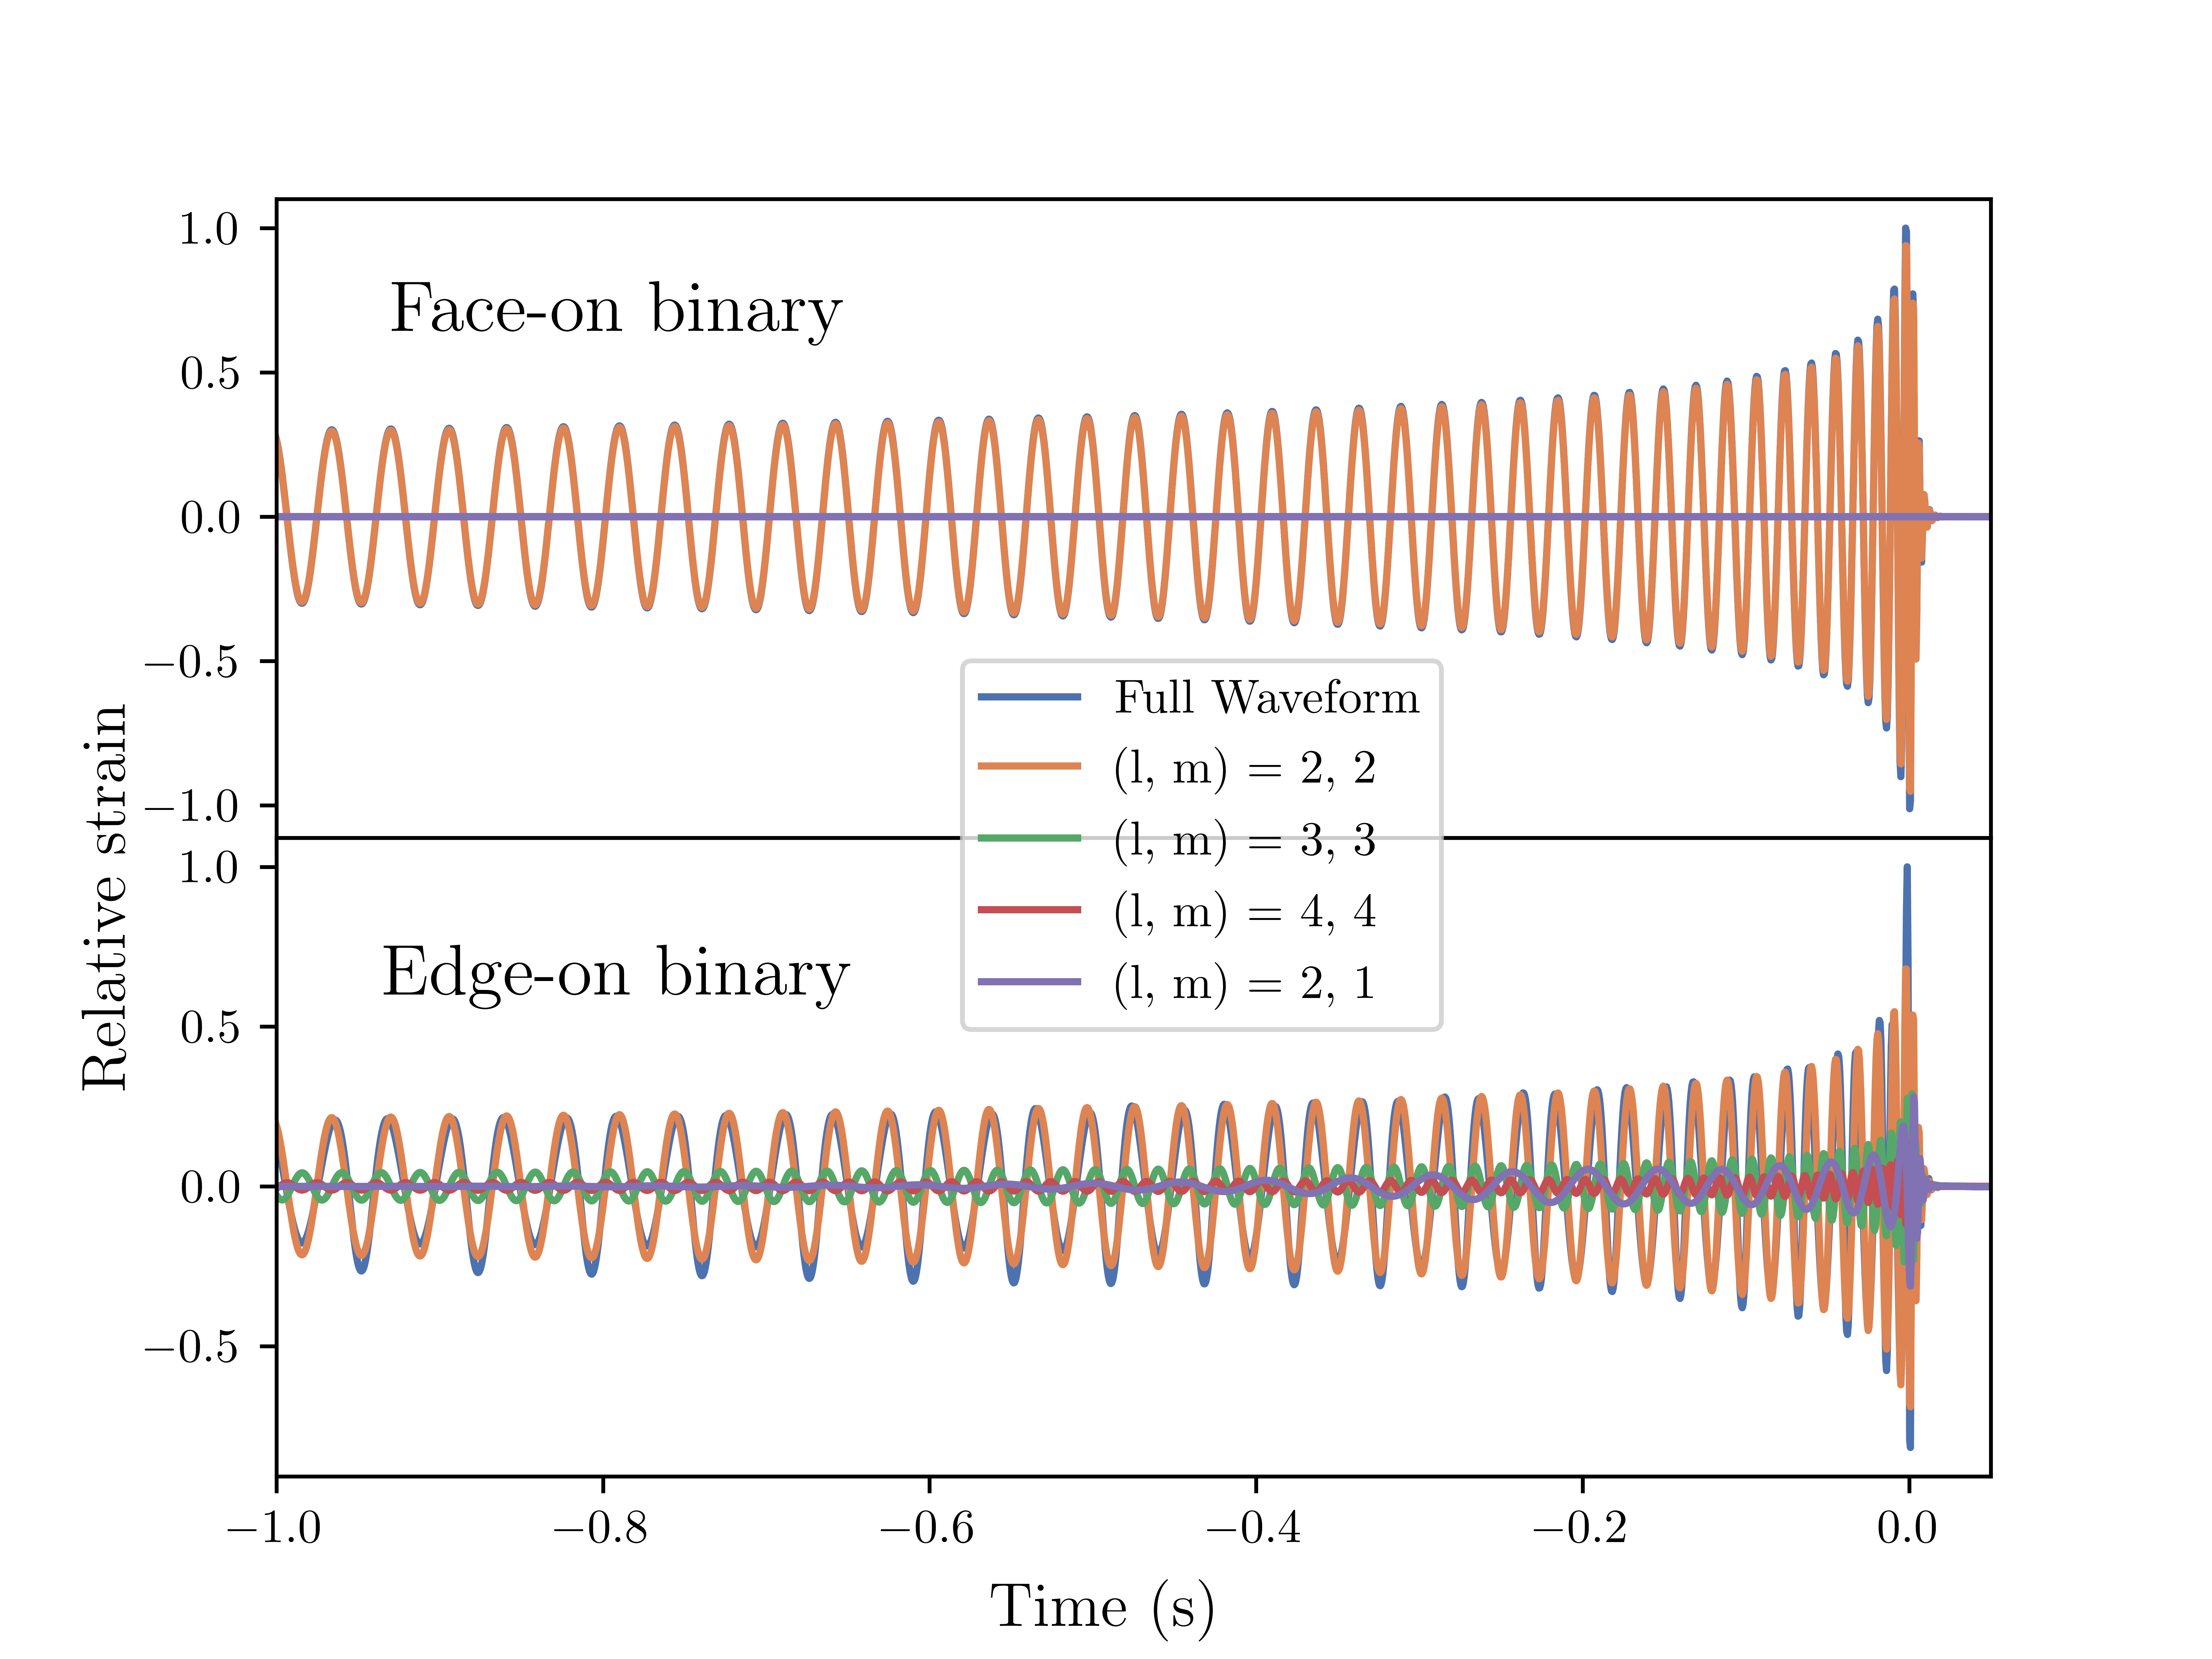
\includegraphics[width=\textwidth]{figures/HM_and_precession/HMs-plots.png}
    \caption{The GW signal from a non-spinning binary with unequal masses $(40,7)M_{\odot}$ is depicted in two distinct orientations: face-on (top) and edge-on (bottom), modeled using the \approximant{IMRPhenomXPHM}. In the face-on binary, the primary (2,2) mode (orange) closely represents the full waveform (blue). However, for the edge-on orientation at an incline, the less dominant modes become more significant, and the (2,2) mode alone fails to fully capture the waveform – necessitating the inclusion of Higher-Order Modes (HMs) for a precise signal depiction.} 
    \label{fig:HMs-plot}
\end{figure}


\begin{figure}
    \centering
    \includegraphics[width=\textwidth]{figures/HM_and_precession/precessing-wf.png}
    \caption{Effect of component spins on the GW signal from an unequal mass $(30,10)M_{\odot}$ binary, shown for -- aligned spins with $\chi_{\text{eff}} = 0.1$ (pink) and randomly oriented spins with $\chi_{p} = 0.5$ (green). Orbital precession in the later case, causes amplitude and phase modulations of the GW signal.} 
    \label{fig:precessing-wf}
\end{figure}


%We denote the spin angular momenta $\textbf{S}_1 = \vec{\chi}_1 m_1^2$ and $\textbf{S}_2= \vec{\chi}_2 m_2^2$.  In the case of aligned-spin systems, the direction of the orbital angular momentum remains fixed and thus, $\textbf{S}_1 \textbf{S}_2$, and $\textbf{L}$ are parallel. In the case of systems with generically oriented spin vectors, the spins of the compact objects couple with the orbital angular momentum which may cause spin-precession. For such systems, the orbital angular momentum $\textbf{L}$ precesses around the nearly fixed total angular momentum $\textbf{J} = \textbf{S}_1 + \textbf{S}_2 + \textbf{L}$; the inclination angle varies over time. The various spin and orientation angles are shown in the Fig. \ref{fig:precessing_angles}. 
%\begin{figure}
%    \centering
%    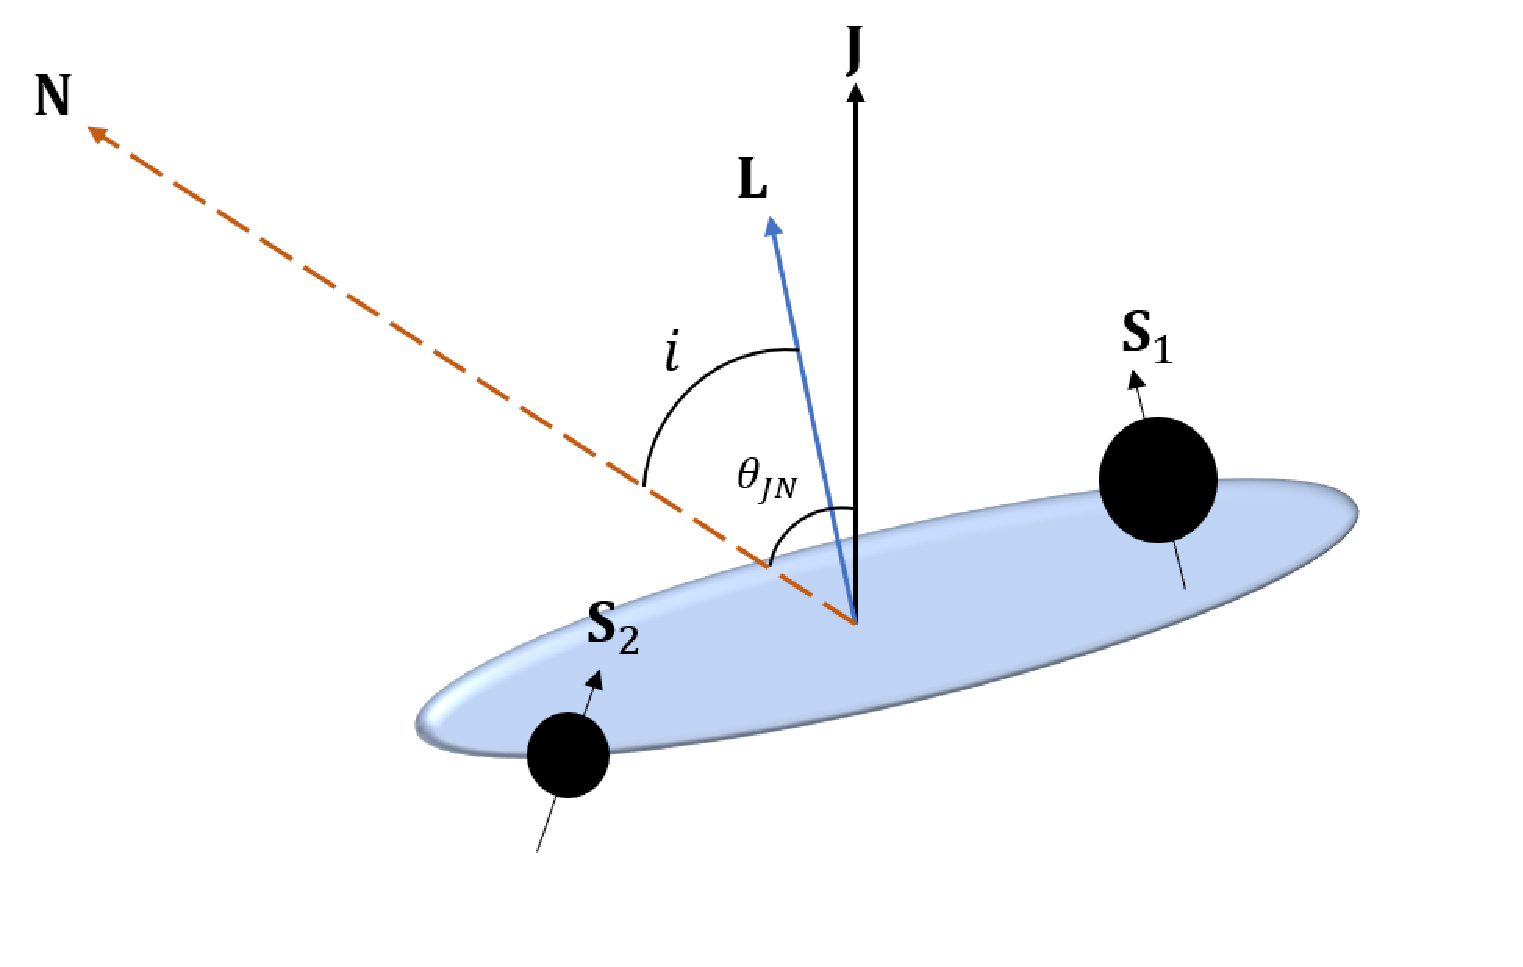
\includegraphics[width=10cm]{figures/HM_and_precession/Precessing_angles.pdf}
%    \caption{The angular momentum vectors for a precessing binary. The inclination angle $\iota$ is defined as the angle between the orbital angular momentum $\textbf{L}$ and the line of sight to the observer $\textbf{N}$. The angle between $\textbf{J}$ and $\textbf{N}$ is denoted as $\theta_{JN}$. Due to spin-orbit coupling, $\textbf{L}$ and $\textbf{S}$ will precess around the approximately fixed $\textbf{J}$.} 
%    \label{fig:precessing_angles}
%\end{figure}

%Precession dynamics cause phase and amplitude modulations to the observed signal. Since precession is caused by the non-alignment of the spins with the orbital angular momentum, to measure the strength of precession, it is common to group the in-plane and parallel spin components. The spin effects are commonly characterized in terms of the two effective parameters \cite{Ajith:2009bn, Schmidt:2014iyl}

%\begin{align}
%    \chi_{\text{eff}} = \dfrac{1}{M}\Bigg(\dfrac{\textbf{S}_1}{m_1}+\dfrac{\textbf{S}_2}{m_2}\Bigg)\cdot\hat{\textbf{L}}, \label{eq:chi_eff}\\
%    \chi_{p} = \dfrac{1}{A_1m_1^2}\max\Big(A_1 S_1^{\perp},A_2 S_2^{\perp}\Big), \label{eq:chi_P}
%\end{align} 

%where, $A_1=2+3q/2$ and $A_2 = 2 + 3/(2q)$, $q$ is the mass-ratio $m_1/m_2$, and $S_i^{\perp}$ is the projection of the spins orthogonal to $\textbf{L}$. The $\chi_{\text{eff}}$ parameter gives us a measure of the spin components parallel to $\textbf{L}$. The four in-plane spin components are averaged over a precessing cycle to obtain an effective $\chi_p$ precession parameter.

\section{ Reference NSBH population } \label{sec:ref_pop}
Since the precession and higher order-mode effects grow with mass-ratio, we choose to study a population of NSBH source extending up to $q = 20$ with the broad priors shown in table~\ref{tab:priors}. We sample the component masses in terms of the detector frame masses $m_{1,2}^{det} = (1+z)m_{1,2}$, where $z$ is the redshift of a source. The redshifted masses are sampled uniformly between $5 M_{\odot} \leq m_1^{det} \leq 30 M_{\odot}$ and $1 M_{\odot} \leq m_2^{det} \leq 3 M_{\odot}$. Working in the detector frame eliminates the redshift dependence in the calculation of signal-to-noise ratio and related metrics (see e.g. sec \ref{sec:metrics}).


We choose the spin directions to be isotropically distributed and the spin magnitudes to be uniform. We assume neutron-stars are slowly spinning with spin-magnitude up to 0.05, and up to one for black-holes. We also assume the sources are isotropically distributed in the sky. The polarization angle, coalescence phase and the cosine of the inclination angle are also uniformly distributed. In total we simulate a population of 50,000 compact-binaries.

In this study, we employ one of the latest models from the phenomenological waveform family \approximant{IMRPhenomXPHM} \cite{Pratten:2020ceb} to generate signals for our fiducial population. This model accounts for generic spins and HMs and includes $(l, |m|) = (2, 2), (2, 1), (3, 3), (3, 2), (4, 4)$ modes. \approximant{IMRPhenomXPHM} has shown consistent results with other waveform models in the recent compact-merger catalogs \cite{LIGOScientific:2021djp, Nitz:2021uxj, Olsen:2022pin}, inference studies of various GW events \cite{Estelles:2021jnz, Krishnendu:2021cyi}, and studies inferring population properties \cite{Tiwari:2021yvr, Zhu:2021jbw}. Thus, the reliability and computational efficiency of \approximant{IMRPhenomXPHM} motivated us to employ this model.  

\begin{table}
    \centering
    \begin{tabular}{c|c}
        Parameter &  Distribution\\
        \hline
        \hline
        $ m_{1}^{det} $ & uniform $\in$ [5.0, 30.0]  $ M_{\odot}$ \\
        \hline
        $ m_{2}^{det} $ & uniform $\in$ [1.0, 3.0] $ M_{\odot} $\\
        \hline 
        $\abs{\chi_{1}}$ & uniform $\in$ [0, 1] \\
        \hline
        $\abs{\chi_{2}}$ & uniform $\in$ [0, 0.05] \\
        \hline
        Spin tilt angles & Isotropic\\
        \hline 
        Sky angles & Isotropic \\
        \hline
        $\Phi_c$ & uniform $\in$ [0, $2\pi$]\\
        \hline
        $\cos{\iota}$ & uniform $\in$ [-1, 1] \\
        \hline
        $\psi$ & uniform $\in$ [0, $2\pi$]
    \end{tabular}
    \caption{ Various source parameters (first column) used in the simulation for the reference NSBH population consisting of 50,000 compact-binaries. The second column shows the distribution used to sample the corresponding parameter.}
    \label{tab:priors}
\end{table}

\section{Measuring the performance of spin-aligned searches}\label{sec:metrics}
Modeled searches with a template bank are bound to lose fraction of signals due to two main reasons -- discreteness of the template bank, and the templates not being the optimal description of astrophysical signals. The loss in sensitivity is quantified using metrics that measure the bank's ability to recover a population of simulated signals. We first define the match between a given template $h_i(\gamma)$ with unknown extrinsic parameters $\gamma$ and a signal $g$ in terms of the overlap $\braket{g|h_i({\gamma})}$ between the two as
\begin{align}
    m(g, h_i) \equiv \mathop{\max}_{\gamma}\Big( \braket{g|h_i(\gamma)} \Big) = \dfrac{1}{\sqrt{2}}\norm{\braket{g|h_i}},
    \label{eq:overlap}
\end{align}
where $i$ is the index corresponding to different templates in a given bank. Computing the match involves maximization over all extrinsic parameters such as $\gamma = (d_L, \iota, \psi, \alpha, \delta, \Phi_c, t_c)$ that are not included in the template bank. Since the intrinsic parameters remain unknown, the match is further maximised over the template bank to obtain the best-fit template to $g$ and its \textit{fitting factor} 
\begin{align}
    \text{FF}(g) = \max_{i} \big(m(g,h_i)\big).
    \label{Eq:FF}
\end{align}

The fitting factor corresponds to the maximum fraction of the absolute signal SNR that can be recovered by a given template bank which ranges $\in [0, 1]$. For instance, a signal with an SNR = 10.0 having a FF of 0.98 can only be detected with a maximum SNR of 9.8. The number of signals detected by a search above some SNR threshold, depends not only on the FF achieved but also on the intrinsic loudness $\sigma(s_i)$ of each signal $s_i$. Varying intrinsic signal loudness leads to an observational bias against intrinsically quieter sources such as highly inclined systems. Such systems might be rarer due to this observational bias and sometimes poor fitting factors may correlate with this bias. We use a metric (introduced in \cite{Buonanno:2002fy}) that takes into account the signal SNR and estimates the number of signal recovered relative to an optimal search that can perfectly match each signal. For a volumetric distribution of $n_s$ sources, the number of signals recovered by a search with a template bank $B$ of fitting factors ($\text{FF}_B$) is proportional to $\sum \limits_{i=0}^{n_s-1} \text{FF}_B^3(s_i)\sigma^3(s_i)$. The fraction of signals recovered relative to an optimal search with $\text{FF} = 1$ is referred as the signal recovery fraction (SRF) and is given by
\begin{align} 
    \text{SRF} \equiv \eta^B = \dfrac{\sum \limits_{i=0}^{n_s-1} \text{FF}^3_B(s_i)\sigma^3(s_i)}{\sum \limits_{i=0}^{n_s-1} \sigma^3(s_i)}.
    \label{eq:SRF}
\end{align}


For a given search, the false-alarm-rate (FAR) can be uniquely mapped to SNR threshold, and detections are often determined by their statistical significance exceeding a false alarm rate threshold. This mapping can vary with different searches as the background distribution of triggers changes. The relative sensitivity between two searches ensuring the same significance is compared at a fixed FAR. Using the threshold $\rho_0$ corresponding to a chosen FAR value, the SRF weighted by the FAR can then be computed using $\eta^{B}/\rho_{0}^3$. As an example, consider two different searches scenarios -- $B$ (dominant mode, aligned-spin) and $B'$ (including precession or HMs) with SNR thresholds $\rho_{\text{ref}}$ and $\rho_{\text{thresh}}$ respectively at a fixed FAR. The relative sensitivity between the two searches is computed according to
\begin{align}
    \beta = \dfrac{\eta^B\rho^3_{\text{thresh}}}{\eta^{B'}\rho^3_{\text{ref}}}
    \label{eq:relative_sensitivity}.
\end{align}

\subsubsection{Aligned-spin template banks for different detectors}
We want to test whether the PSD (noise curve) of a detector have significant impact on the template bank and thus the detectability of signals. Since the PSD influences the distribution of templates -- for a detector with wider sensitive bandwidth, a template can accrue greater phase mismatch with a slight variation in the parameters and will result in increased number of templates. Future detectors are expected to have larger bandwidths, as such better sensitivity at lower frequencies increases the duration of signal in the sensitive band of the detector. Due to this template banks for future observatories are expected to have up to an order of magnitude larger template banks than the ones for the current observatories. The expected noise curves for the Advanced LIGO, $A+$, LIGO Voyager and CE are shown in the Fig. \ref{fig:PSDs}.  

\begin{figure}
    \centering
    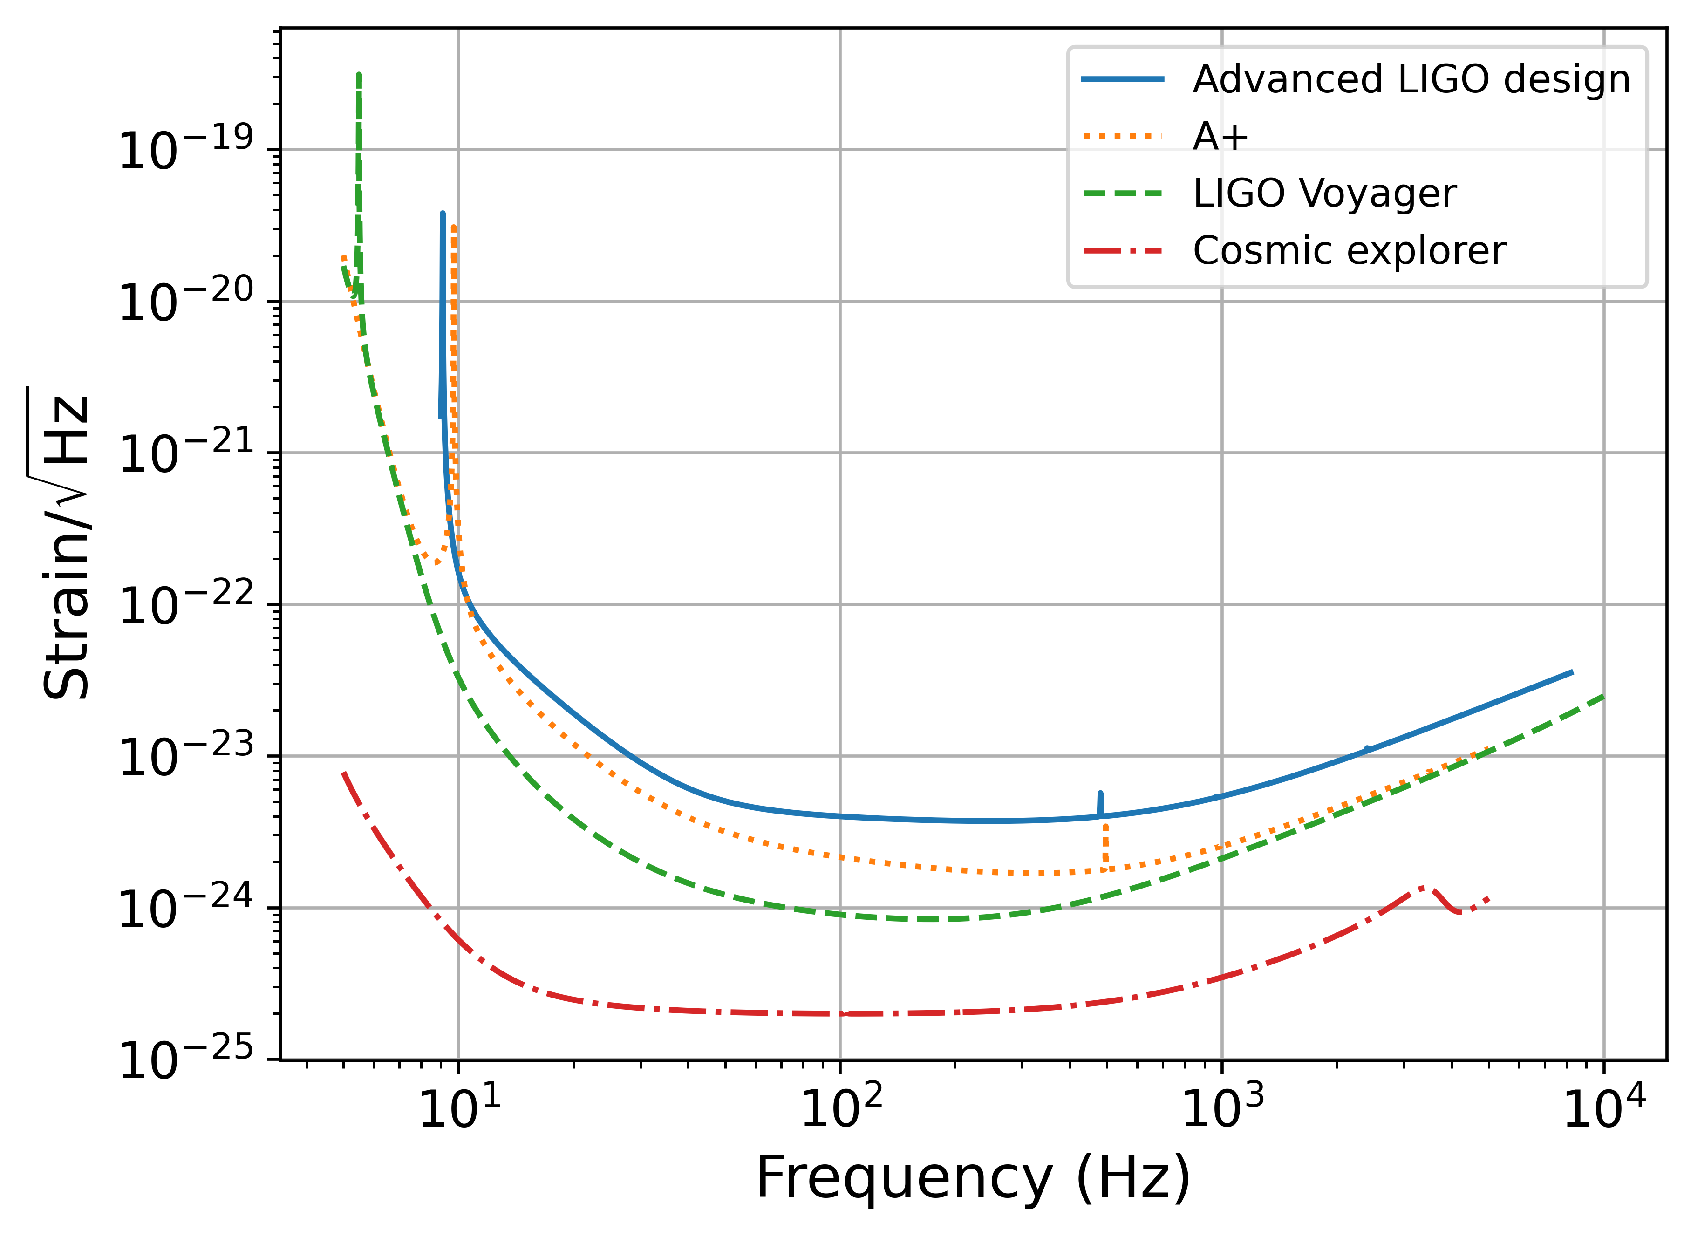
\includegraphics[width=\linewidth]{figures/HM_and_precession/PSDs.pdf}
    \caption{A comparison of the noise amplitude spectral density (ASD) of each detector configuration used in this study. Aligned-spin template banks are generated for each noise curve using the appropriate $f_{low}$. } 
    \label{fig:PSDs}
\end{figure}

To test this faithfully, we use the lower frequency cutoff appropriately for the template banks respective to each detectors considered. Both Advanced LIGO and A+ observatories are expected to be sensitive down to 15 Hz. LIGO Voyager is anticipated to be sensitive from 10 Hz upwards. Cosmic Explorer is predicted to be sensitive down to 5Hz; however, in \cite{Lenon:2021zac} the authors find $99.53\%$ of the signal SNR will be retained at a lower frequency cutoff = 7Hz and Doppler modulations can be neglected from this lower frequency.

In this work, we generate dominant mode only, aligned-spin banks by sampling the 4D $(m_1, m_2, \chi_{1z}, \chi_{2z})$ parameter space using a stochastic sampling method \cite{Harry:2009ea,Babak:2008rb}. We use \approximant{SEOBNRv4\_ROM} model and use the appropriate lower frequency cutoff $f_{low}$ for a given sensitivity curve. All the template banks are generated with an average mismatch of $< 1\%$. 


\section{Assessing the loss due to omitting HMs and precessional effects}\label{sec:results}
In this section we estimate the loss in sensitivity for a dominant-mode, aligned-spin search to our reference NSBH population. We sample the source parameters according to the Table \ref{tab:priors} and generate precessing signals with HMs. To study the effects of precession and HMs in isolation, we create two additional sets of signals -- precessing signals with only the dominant mode, and nonprecessing signals with HMs by setting the in-plane spin components to zero which ensures consistent $\chi_{eff}$ distribution. To validate the expected recovery of signals similar to the dominant mode aligned spin templates, we also generate nonprecessing signals with only the dominant mode. In summary, we create four different classes of signals (Table \ref{tab:injection_classes}) -- nonprecessing dominant mode only (baseline), nonprecessing with HMs,  precessing dominant mode only, and precessing with HMs. We use \approximant{IMRPhenomD} \cite{Husa:2015iqa, Khan:2015jqa} a high performant model to generate the baseline injections; in our population of aligned-spin signals, without HMs we expect the mismatch effects due to the discreteness of the template bank to dominate over the inaccuracy of the waveform model ~\cite{Pratten:2020fqn}. For all the other classes we use \approximant{IMRPhenomXPHM} to generate the signals. All signals are projected to the detector frame by linearly combining the two polarizations with the antenna pattern functions as per Eq. (\ref{Eq:Detector_response}). 

\begin{table}
    \centering
    \begin{tabular}{c|c|c}
         Class & Type & Waveform model \\
              &        &    \\
        \hline 
        \hline
       I & nonprecessing dominant mode only& \approximant{IMRPhenomD} \\
       \hline
       II & nonprecessing with HMs & \approximant{IMRPhenomXPHM} \\
       \hline
       III & precessing dominant mode only & \approximant{IMRPhenomXPHM} \\
       \hline
       IV & precessing with HMs & \approximant{IMRPhenomXPHM} \\
    \end{tabular}
    \caption{Four different classes of signals used in this work to study the impact of the missing features. The baseline signals (type I) are simulated using a nonprecessing waveform model without the HMs \approximant{IMRPhenomD}, while all the other types are generated using an updated model which accurately models precession and HM effects \approximant{IMRPhenomXPHM} \cite{Pratten:2020ceb}.}
    \label{tab:injection_classes}
\end{table}

We have made all source code and the results discussed in this section such as fitting factors and signal recovery fractions publicly available at \cite{github}. The repository also contains the scripts that were used to create the graphics shown in this paper. 


\subsection{Signal-to-noise recovery}
 We calculate the distribution of fitting factors (fraction of SNR recovered by a reference aligned-spin search) for each class of signals. The cumulative distributions of the FFs for all classes of signals is shown in Fig. \ref{fig:design_CDF}. Since the templates and baseline injections belong to the same class of signals, as expected, we find the average FF is close to unity. However, the dominant mode, aligned-spin template bank shows long tails of poor FFs for signals with precession or HM effects; FF values down to $\sim0.5$ for precessing signals and down to $\sim0.65$ for nonprecessing signals with HMs. Higher-modes alone do not reduce the FF distribution as much as precession alone (without higher-modes). We expect the distribution of FFs to vary as a function of component mass, spin, and binary orientation, due to the non-uniform impact of precession and higher-order modes; we will study this variation in the following sections.

\begin{figure}
    \centering
    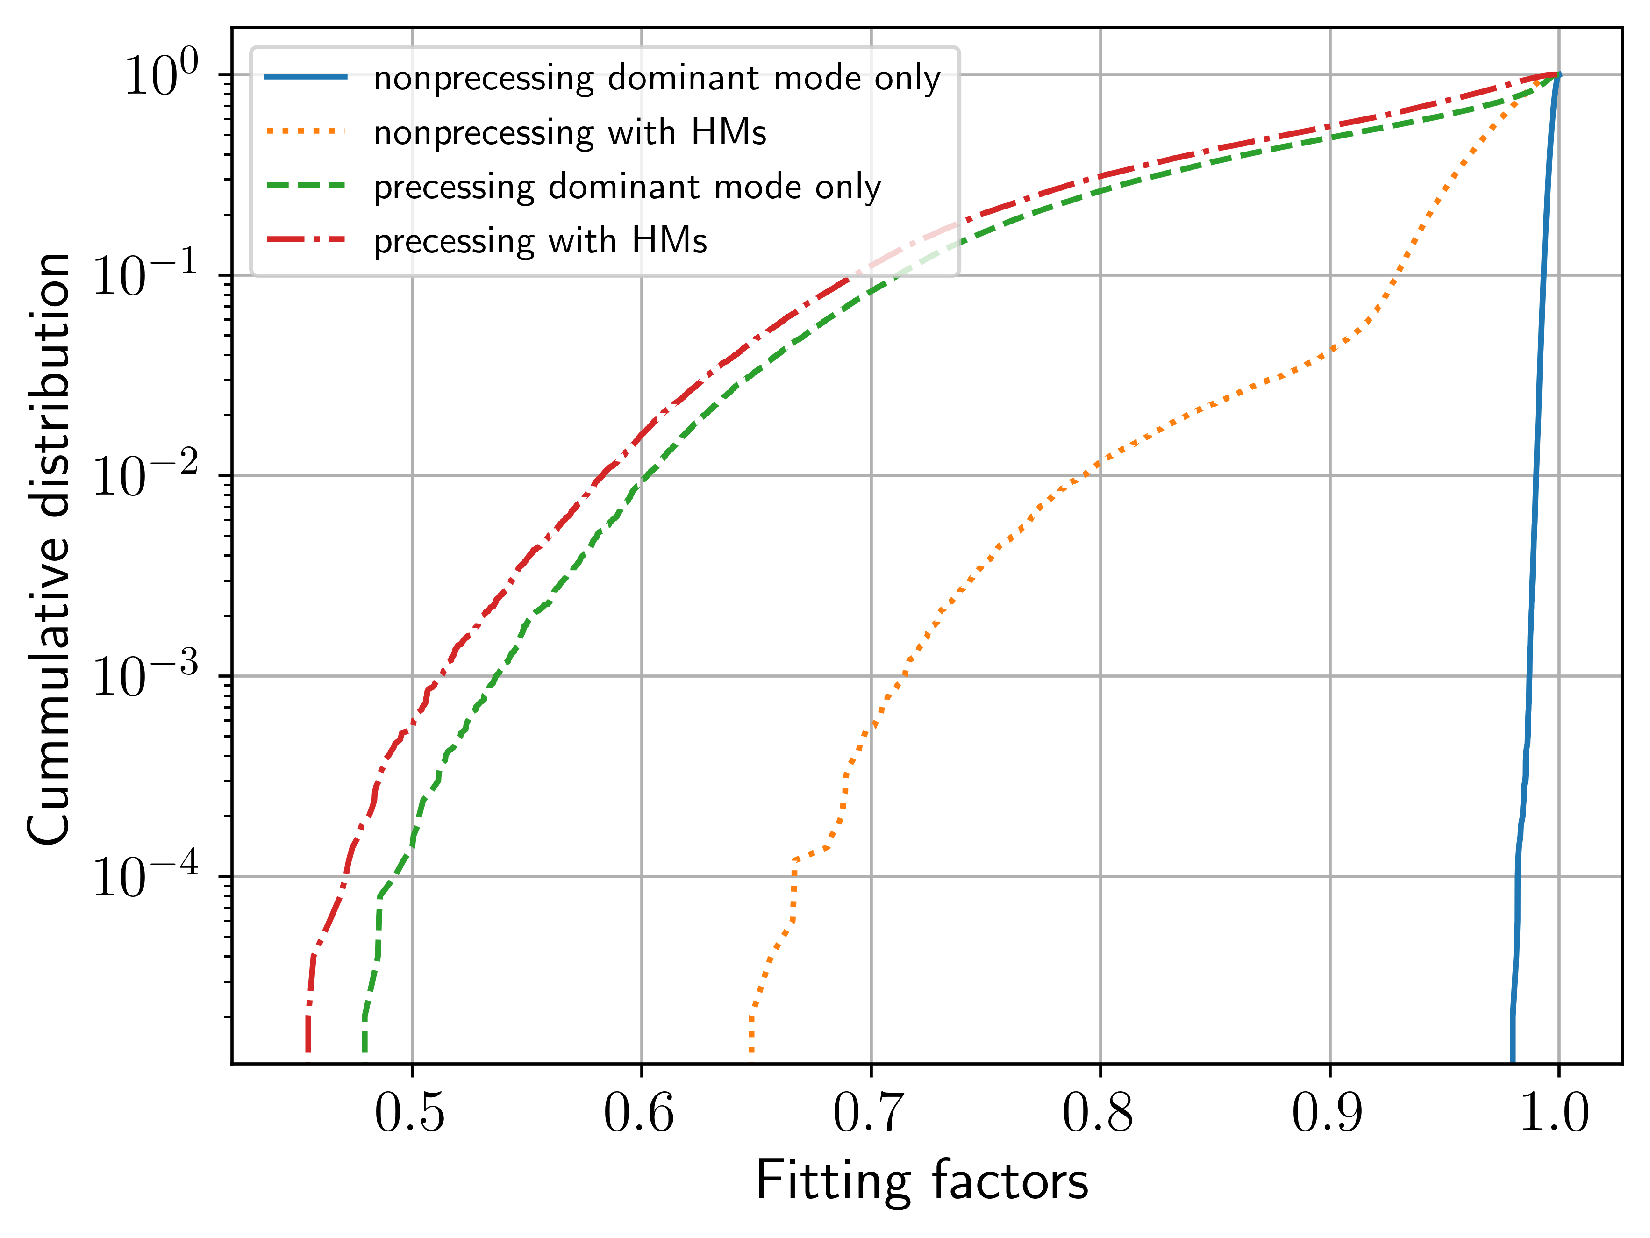
\includegraphics[width=\linewidth]{figures/HM_and_precession/design_CDF.pdf}
    \caption{Cumulative distribution of the FFs for different classes of signals obtained using a dominant mode, aligned-spin template bank using the Advanced LIGO design noise curve. The blue curve confirms the expected number of signals recovered with high FFs above the average minimum match ($< 1\%$). We find long tails of poor FFs for signals with precession or HMs. Also, note precession effects dominate the FFs.}
    \label{fig:design_CDF}
\end{figure}

\subsubsection{Component Masses}
 The impact of both precession and HMs on the observed gravitational-wave signal grows with the mass-ratio of the system. In Fig. \ref{fig:FF_m1m2} we show the population-averaged FF for all classes of signals for the Advanced LIGO design sensitivity as a function of $(m_1^{det}, m_2^{det})$. The top left subplot confirms the intended recovery of baseline signals throughout the parameter space. For nonprecessing signals with HMs (top right), we notice only a slight drop in the FF values (up to $\sim$ 8\%). With precessing signals (bottom row) we observe a clear trend in the FF distribution; FFs decrease with increasing mass-ratio (top-left to bottom-right). We find the average fractional loss in FFs can be as high as $\sim 15 - 22\%$ for highly asymmetric precessing systems. By comparing the subplots in the bottom row from Fig. \ref{fig:FF_m1m2}, we infer the precession effects dominate the FF distribution. These results confirm that HMs and precession effects grow stronger with increasing mass-ratios of compact-binaries.

\begin{figure*}
    \centering
    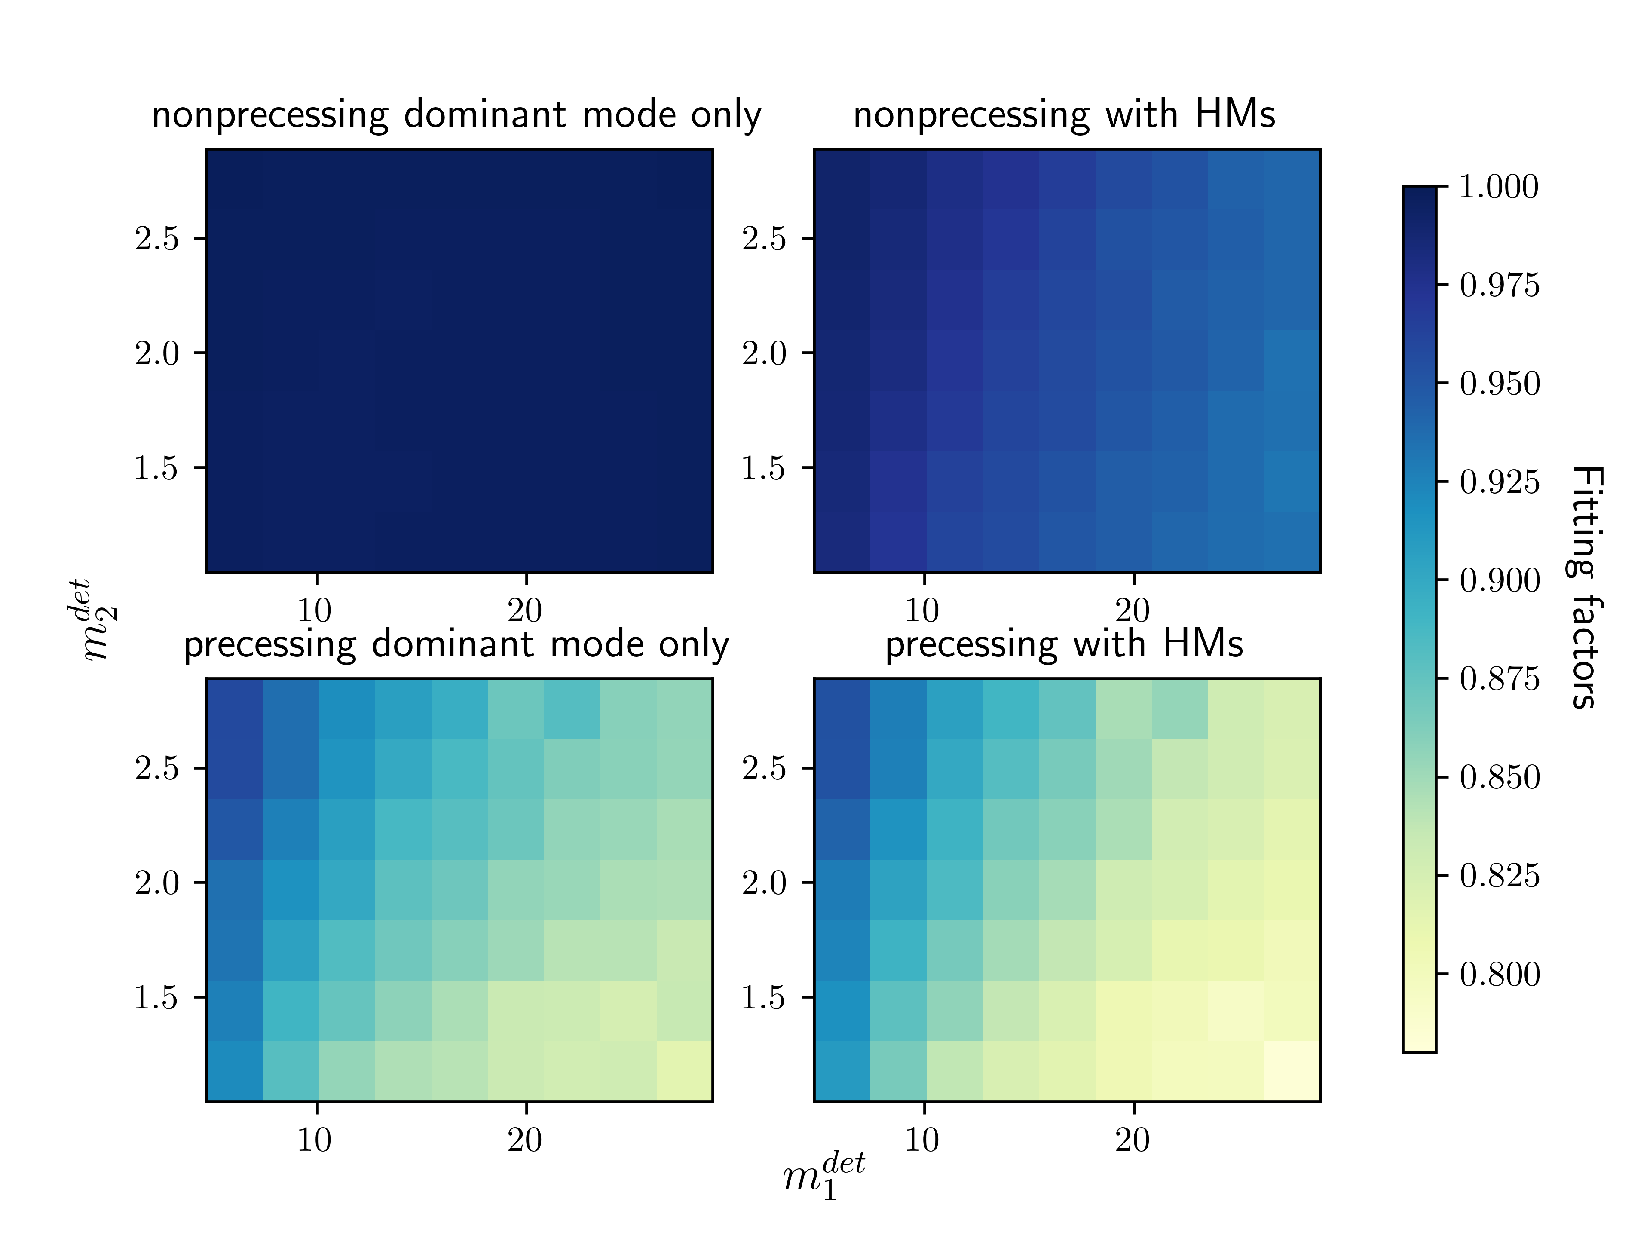
\includegraphics[width=13cm, height=10cm]{figures/HM_and_precession/aLIGO_FF_masses.pdf}
    \caption{Average fitting factors for a population of simulated NSBH signals distributed across the ($m_1^{det}, m_2^{det}$) space obtained using a dominant mode, aligned-spin template bank and assuming the Advanced LIGO design sensitivity. We show the FFs for four different class of signals -- nonprecessing dominant mode only(top-left), nonprecessing with HMs (top-right),  precessing dominant mode only (bottom-left) and  precessing with HMs (bottom-right). We observe a reduction in FFs (fractional loss in observable SNR) up to $8\%$ for signals with HMs, and up to $20 \%$ for precessing sources. Notice the precession effects dominate the FF distribution over HMs.}
    \label{fig:FF_m1m2}
\end{figure*}

\subsubsection{Orientation of the binary}

The orientation of a binary is generally characterized in terms of the inclination angle $\iota$ between $\textbf{L}$ and $\textbf{N}$. However, in the case of precessing system $\iota$ changes over time. To study the dependence of FFs on the orientation of the binary, we instead estimate the distribution in terms of $\theta_{JN}$ evaluated at a reference frequency $f_{ref}$ = 100 Hz of the GW emission; $\theta_{JN}$ will typically be stable over the duration of the signal. In Fig. \ref{fig:FF_orientation} we show the binned population-averaged FF distribution as a function of $(q,\theta_{JN})$ for nonprecessing signals with HMs (left) and dominant mode precessing signals (right). Similar to Fig. \ref{fig:FF_m1m2}, we confirm both HMs and precession effects grow stronger with increasing mass-ratios. Importantly, FFs decreases as the binary moves away from face-on/off configuration and reaches minimum at the edge-on configuration. This is expected because the dominant mode is faintest at $\iota=\pi/2$ and also various higher-order modes have significant contribution for edge-on binaries. 
For the non-precessing, dominant-mode only sources, a maximum loss in FFs up to $10\%$ for highly asymmetric nearly edge-on binaries. In the right plot, we observe much larger losses in FFs for precessing systems. We observe minor losses up to $\sim 10\%$ even for nearly equal-mass systems. For precessing systems with large mass-ratios ($q > 10$), we observe losses in FFs up to $\sim 18-23\%$ for edge-on and up to $\sim 16\%$ for face-on/off binaries.

\begin{figure}
    \centering
    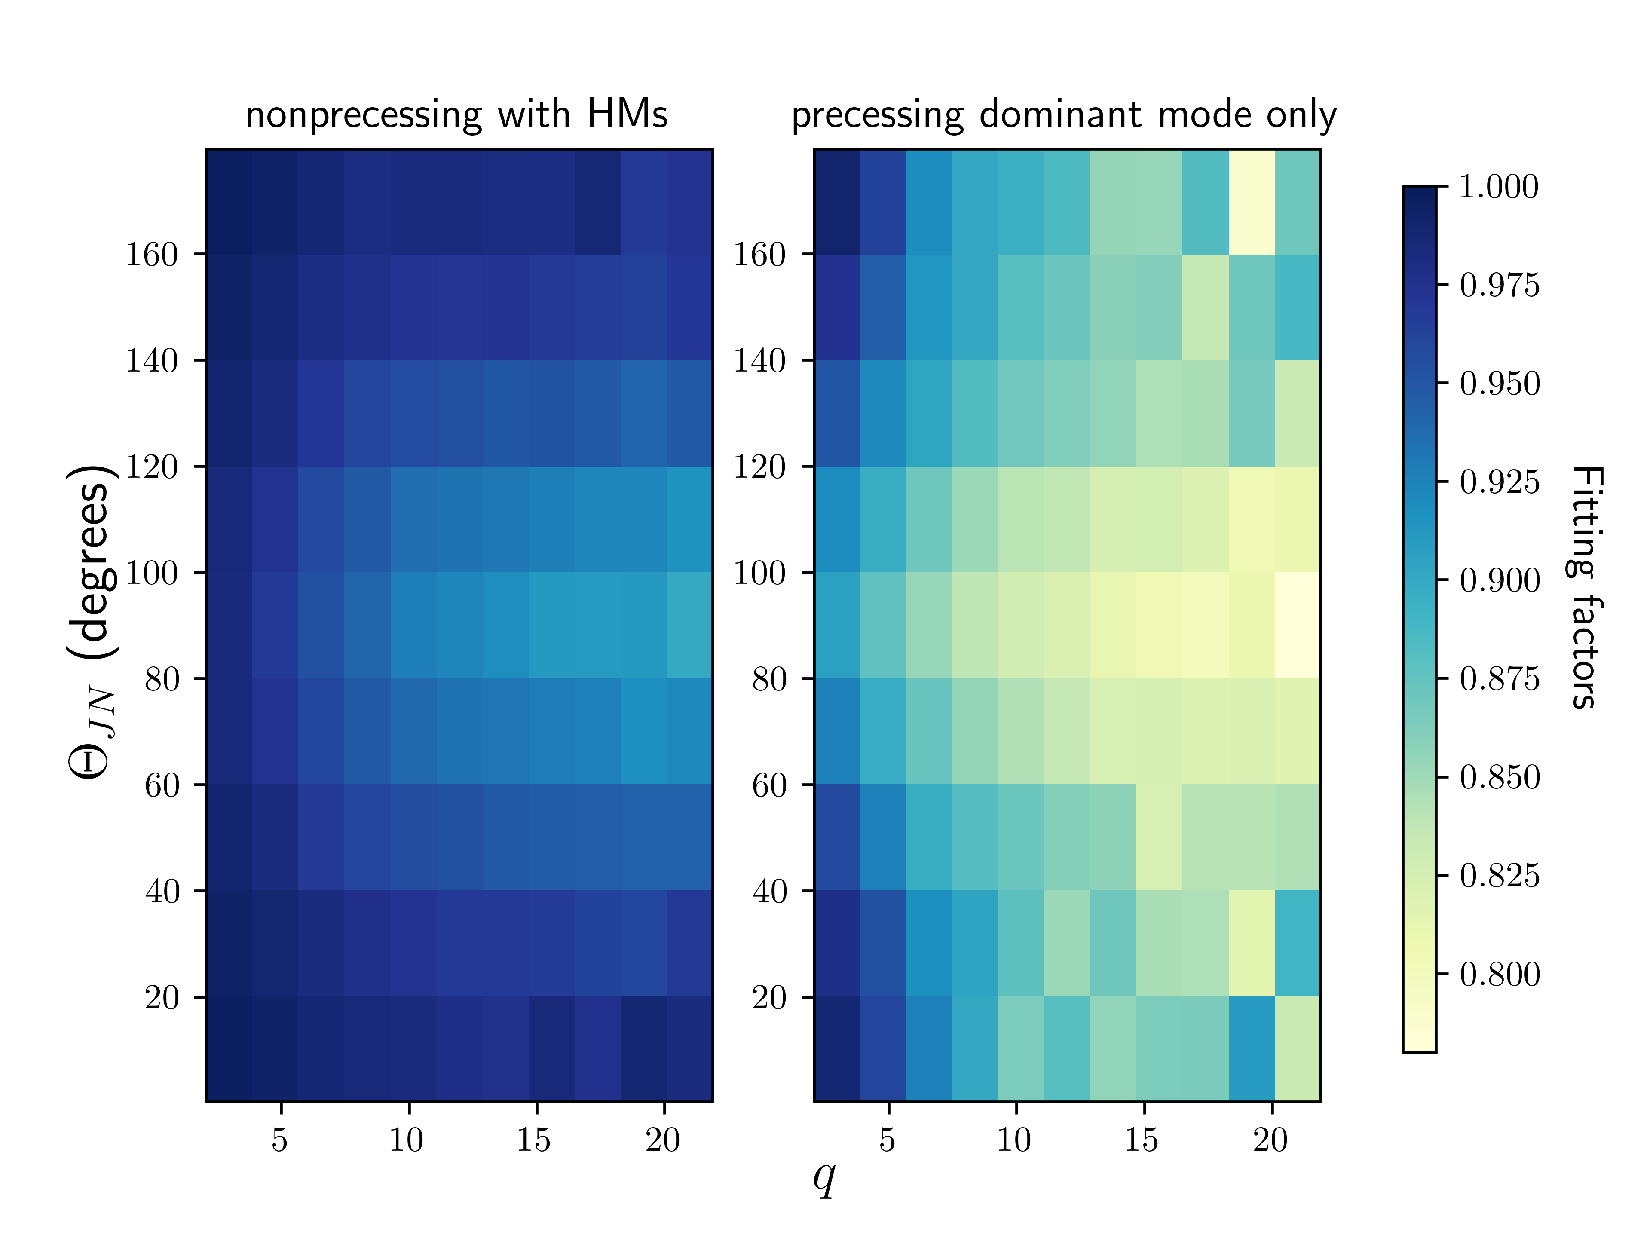
\includegraphics[width=\linewidth]{figures/HM_and_precession/aLIGO_FF_orientation.pdf}
    \caption{ The average FFs as a function of ($q, \theta_{JN}$) at $f_{ref} = 100$ Hz, for a simulated population of signals containing HMs  (left) and precession with only the dominant mode (right). We observe larger losses in FFs for precessing signals than for signals with HMs. We notice a trend of decreasing FFs when the source orientation changes from face-on/off to edge-on or when the mass-ratio increases.}
    \label{fig:FF_orientation}
\end{figure}

\subsubsection{Component spins} \label{component-spins}
 The ability for in-plane spin to cause precession, is typically measured in terms of the effective precession $\chi_P$ parameter (Eq. (\ref{eq:chi_P})). The binned population-averaged FF distribution as a function of $(\chi_P, \theta_{JN})$ is shown in Fig. \ref{fig:chi-theta}. We use two classes of signals, precessing signals without HMs (left), and with HMs (right). As expected from Fig. \ref{fig:FF_orientation}, for a fixed value of $\chi_P$ we observe the same trend across $\theta_{JN}$ -- decreasing FFs as the binary shifts away from face-on or face-away configuration. As the precession increases (left to right), the FFs decrease; this occurs because precession causes strong amplitude and phase modulations in the signal which which may not be captured by nonprecessing templates. The nearly identical subplots suggest insignificant impact from the HMs. For slightly precessing sources ($\chi_P < 0.5$), we find $\sim 12-20\%$ loss in FFs. For highly precessing systems the loss in FFs can be up to $\sim 28\%$ for edge-on and up to $\sim 20\%$ for face-on binaries. The difference between the FFs for the two considered signal classes gives the residual impact on FFs from HMs only where the maximum difference obtained is $4\%$. As a function of $(\chi_P, \theta_{JN})$ the difference of FFs shows a similar behaviour as Fig \ref{fig:FF_orientation}; poor values for increasing inclination. Also, the value gets smaller as $\chi_P$ increases, indicating dominating precessional effects.

 \begin{figure}
    \centering
    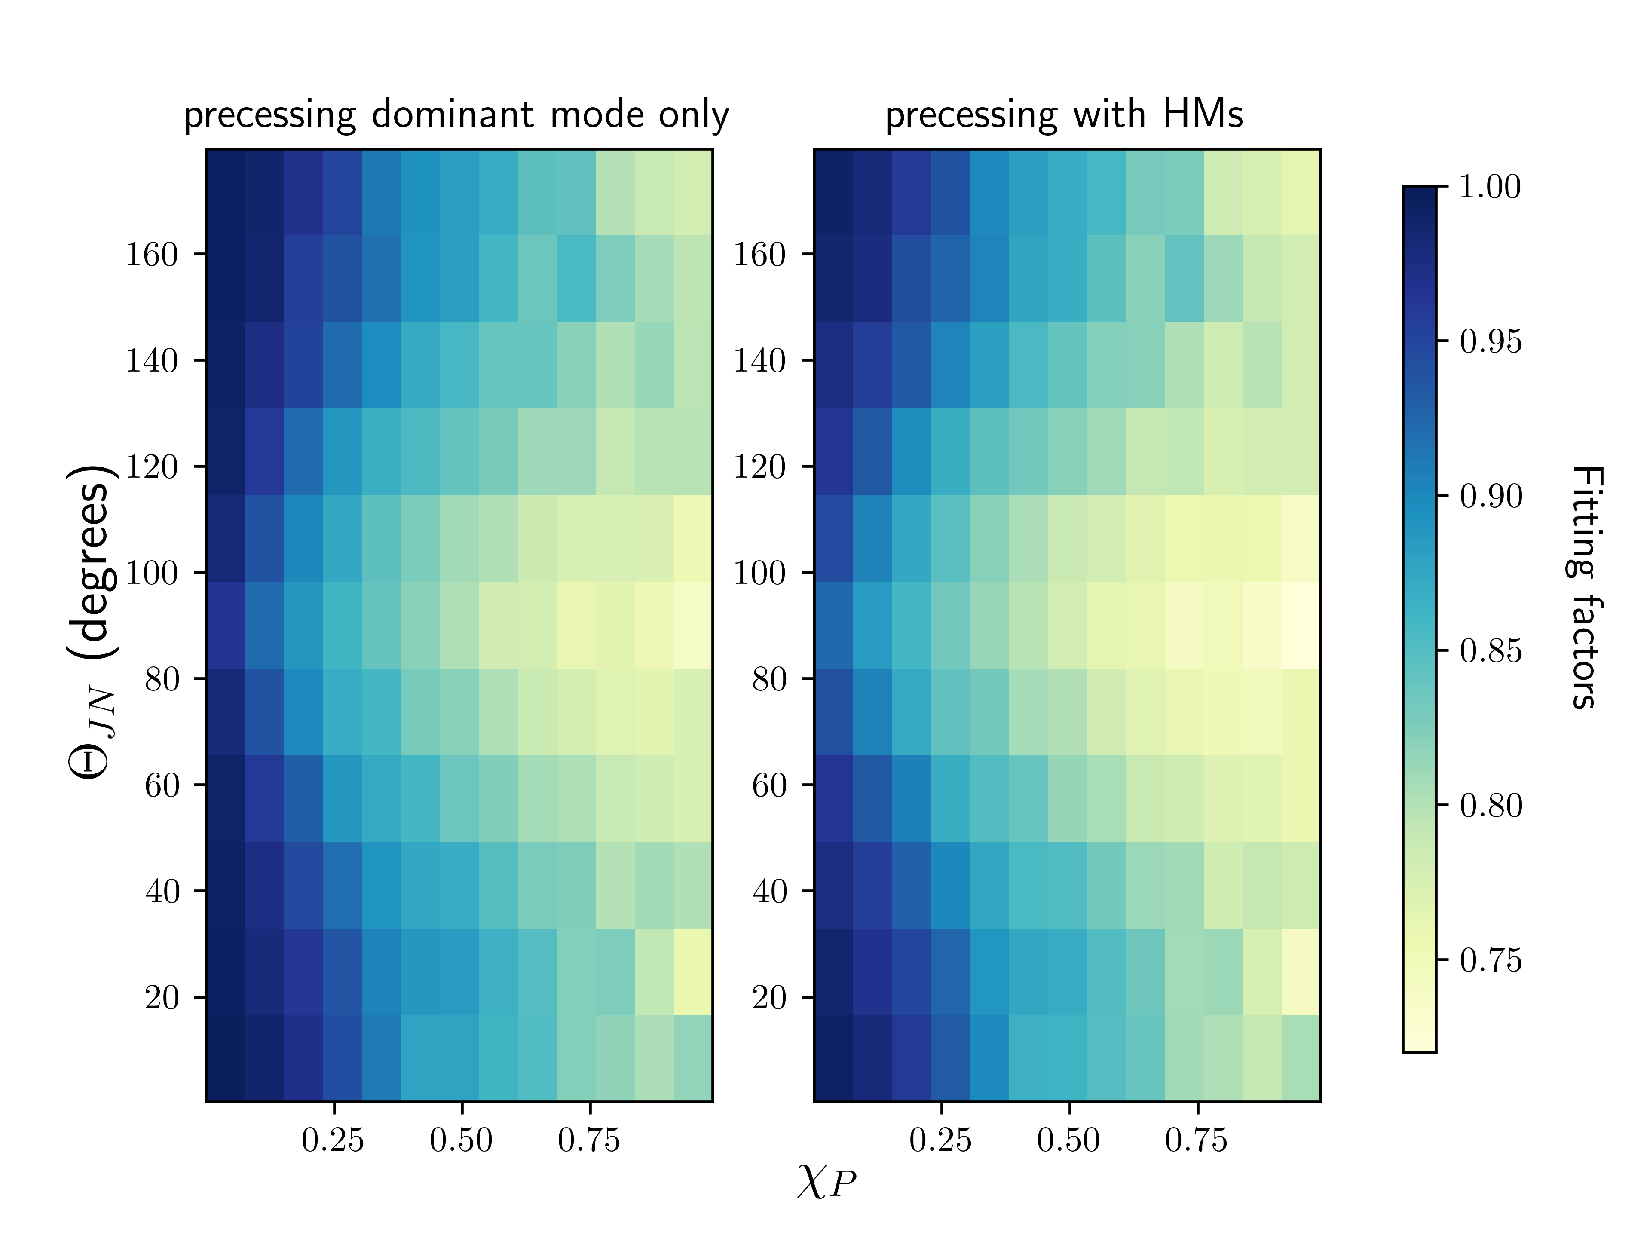
\includegraphics[width=\linewidth]{figures/HM_and_precession/aLIGO_FF_spins.pdf}
    \caption{ The average FFs as a function of effective precession and source orientation $(\chi_p, \theta_{JN})$, for precessing signals without HMs (left) and with HMs (right). Due to the dominance of the precessing effects, there is no significant difference between the two subplots. The  FFs decrease as the effective precession increases and the source becomes closer to edge-on, up to an average loss of $\sim20-30\%$ in SNR.}
    \label{fig:chi-theta}
\end{figure}

\subsubsection{Comparing different detector configurations}

Fitting factor depends on the noise curve (PSD) and the lower frequency $f_{low}$ used to compute matches as per equations (\ref{eq:overlap}) and (\ref{Eq:FF}). We study the variation in FF distribution across four different detector configurations by using their respective noise curves (as shown in Fig. \ref{fig:PSDs}) and the appropriate $f_{low}$. 
In the Fig. \ref{fig:FF_diffPSDs}, we show the distribution of the FFs across ($m_1^{det}, m_2^{det}$) space for all detector configurations. To aid in comparison, we show the FFs for only the precessing signals with HMs case. There is no significant difference between FFs for the different detectors and detector configurations. The change in the noise curve between Advanced LIGO though Cosmic Explorer is not large enough to significantly change the key results.

\begin{figure*}
        \centering
        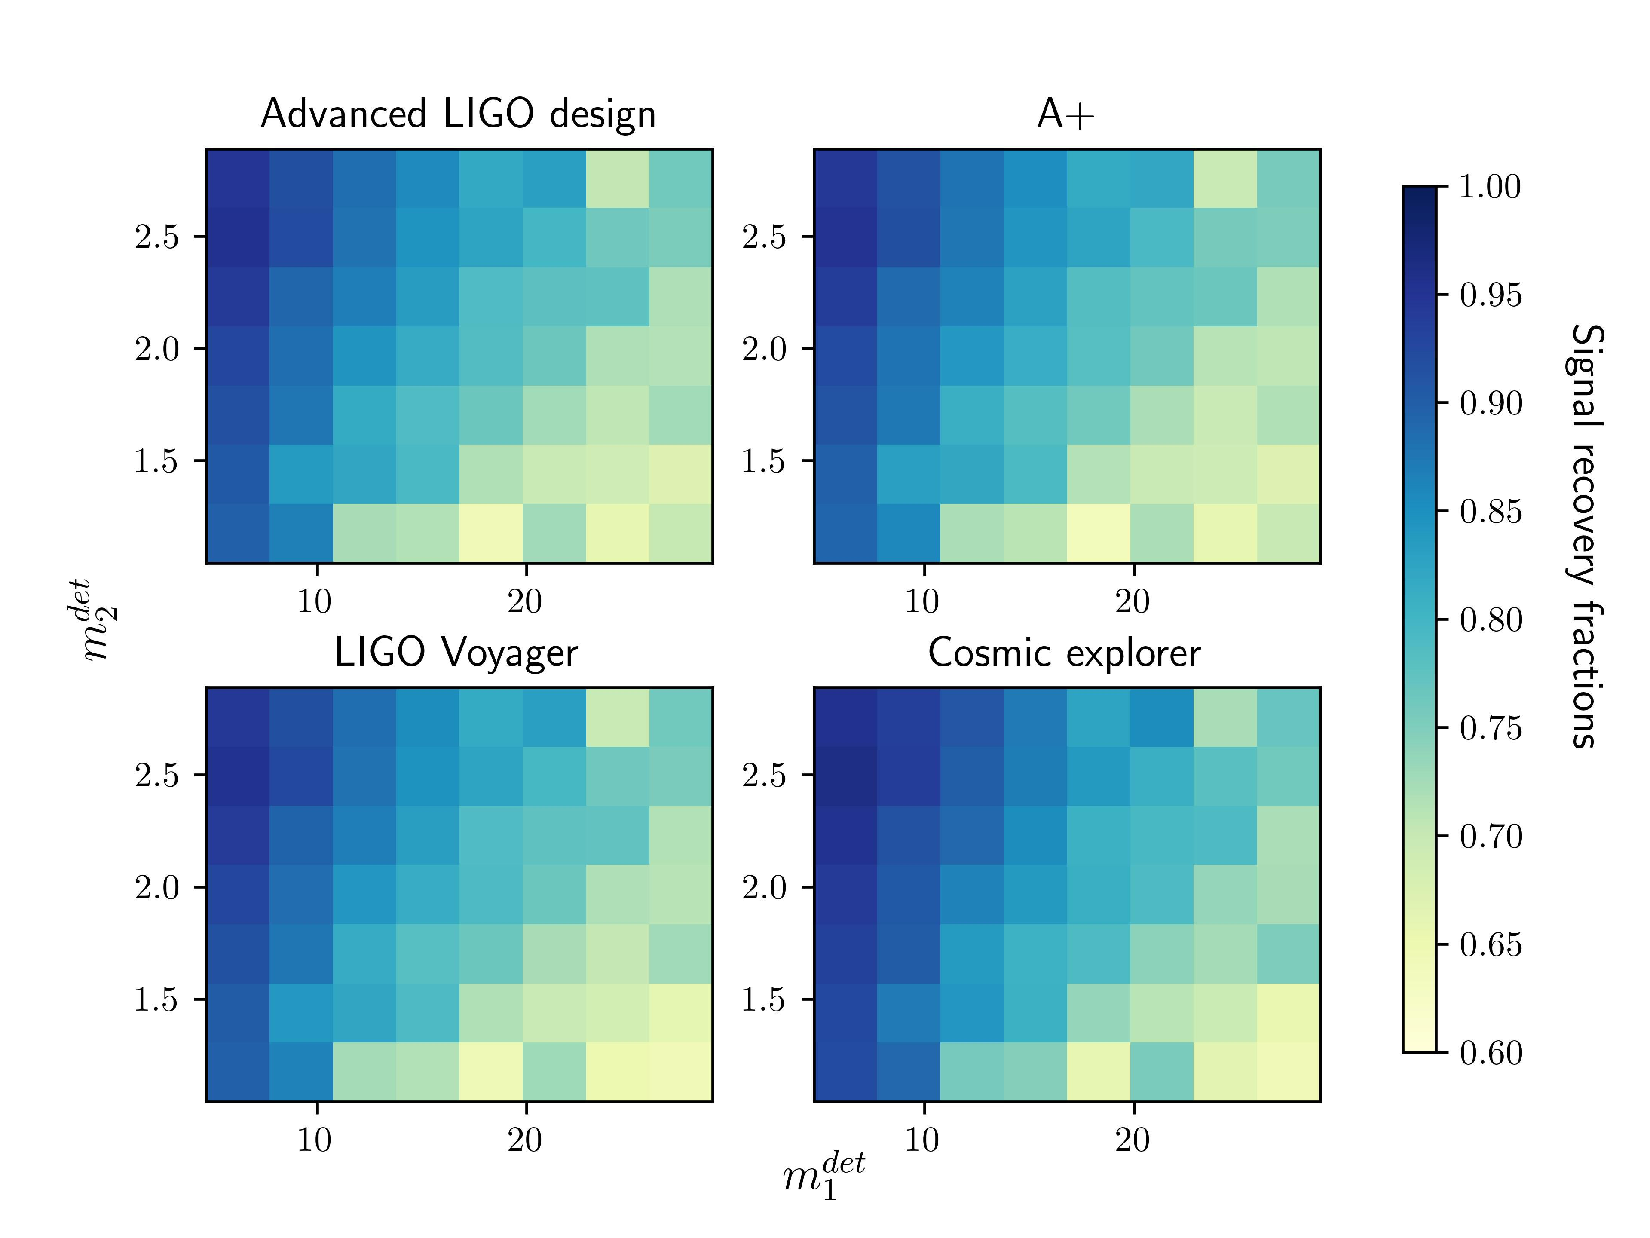
\includegraphics[width=13cm, height=10cm]{figures/HM_and_precession/SRF_diffPSDs.pdf}
        \caption{ FF distribution for precessing sources with HMs as a function of $(m_1^{det}, m_2^{det})$ for different detector configurations. We can see that the results are not strongly dependent on the noise curve.}
        \label{fig:FF_diffPSDs}
\end{figure*}

\subsection{Number of Detectable Sources}

In the previous section, we have studied the distribution of SNR fraction recovered by an aligned-spin search with respect to an idealized search that could recover all of a signal's SNR. 
A real search will have an observational bias towards signals which are louder in comparison to others, which is not taken into account in the FF distribution. We can estimate the fraction of signals (SRF) that would instead be detected by an aligned-spin search w.r.t. an idealized search assuming a fixed SNR detection threshold.
In Fig. \ref{fig:SRF_diffPSDs} we show the distribution of the SRF for precessing signals with HMs as a function of $(m_1^{det}, m_2^{det})$ for all four detector configurations. We notice a similar trend as the FF distribution; decreasing SRF with increasing mass-ratio of the binary. We find dominant mode aligned-spin template banks will miss up to $\sim 13\%$ of nonprecessing signals with HMs (not shown in the figure) and up to $\sim 40\%$ of the precessing systems assuming our fiducial population. These results hold for each detector configuration.

\begin{figure*}
        \centering
        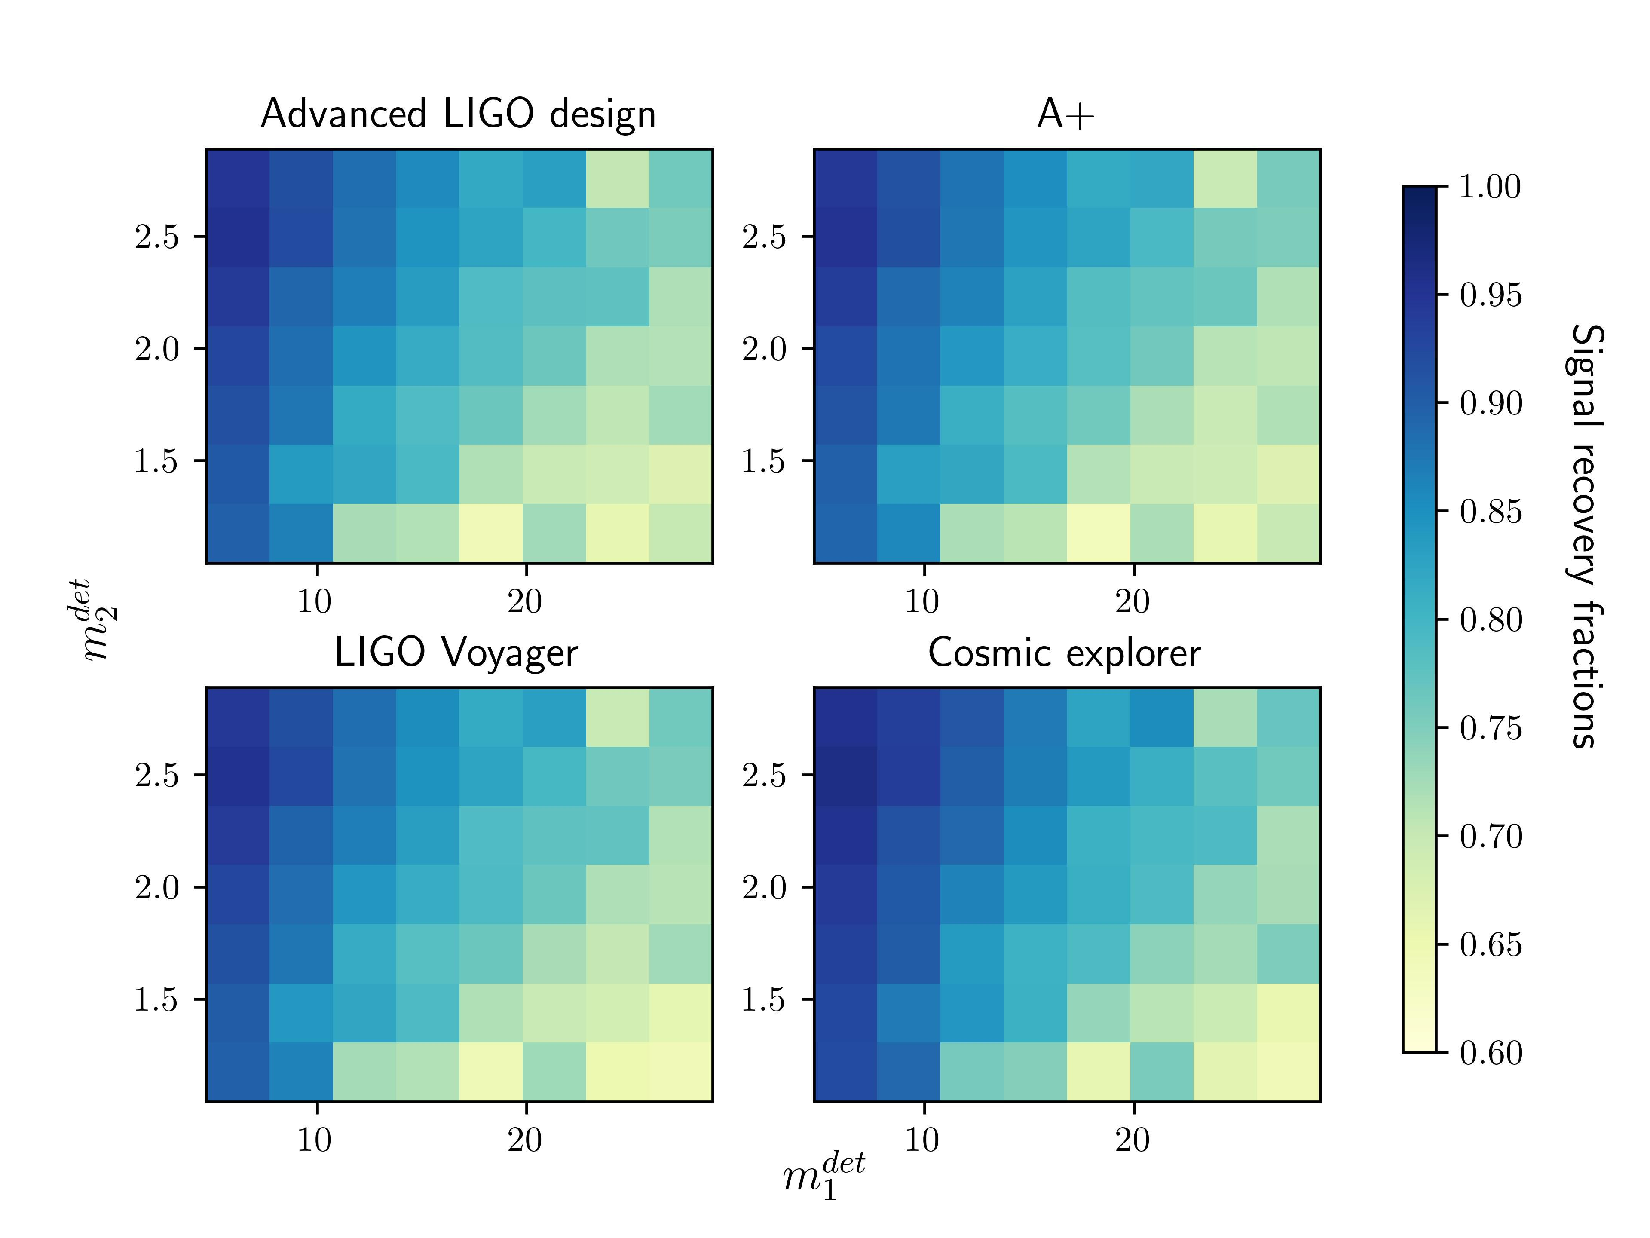
\includegraphics[width=13cm, height = 10cm]{figures/HM_and_precession/SRF_diffPSDs.pdf}
        \caption{The fraction of detectable precessing sources (with HMs) at a fixed SNR threshold (SRF) $m_1^{det}-m_2^{det}$ for different detector configurations. We observe a similar trend as the FF distribution in Fig. \ref{fig:FF_diffPSDs}; the SRF decreases as the mass-ratio increases and there is no significant change in sensitivity across various detector configurations. We observe a loss of up to $40 \%$ for precessing sources ($13\%$ for non-precessing sources) with higher modes included.}
        \label{fig:SRF_diffPSDs}
\end{figure*}

In practice, a real search that could incorporate the effects of precession and higher-order modes
would incur a trials factor relative to the aligned-spin search; this has subdominant impact on the achievable sensitivity. To give an idea of the magnitude of this effect, we can approximate the relative sensitivity at a fixed false alarm rate, rather than at a fixed SNR threshold (see Eq. (\ref{eq:relative_sensitivity})). As a rough estimate, we take the appropriate $\rho_{\text{thresh}}$, chosen to correspond to a given false alarm rate, from previous works which study developing HM~\cite{Harry:2017weg} and precessing searches~\cite{Harry:2016ijz} as shown in the Table \ref{tab:FAR}. 
Typically less than 1 in every 100 or 1000 years are used to claim a significant event \cite{Usman:2015kfa, Messick:2016aqy}. We evaluate the relative sensitivity $\beta$ at these FARs of an aligned-spin search w.r.t. three different idealized searches: a HM search, a precessing, dominant-mode search, and a precessing higher-mode search. Since, precession effects dominate, we use the same effect threshold for the precessing cases.

In Fig. \ref{fig:aLIGO_weightedSRF}, we show the sensitivity relative to all three types of searches using the Advanced LIGO design noise curve as a function of ($m_1, m_2$). Parameter regions where the relative sensitivity is $\leq 1$ depicts regions where aligned-spin search is less sensitive than the more advanced, ideal search. When searching for nonprecessing binaries, the aligned-spin bank is more sensitive than a naive search including HMs on average. But, an aligned-spin search loses up to $\sim 25\%$ of highly precessing ($\chi_P > 0.5$) and highly asymmetric ($q > 6$) NSBH binaries averaged over our fiducial population. We further classify sources based on separate mass-ratio regions, with $q\in$ [2, 5], [5, 10], [10, 15] or [15, 20], and plot the relative sensitivity for all the sub-populations as a function of ($q, \chi_p$) (left) and ($\chi_p, \theta_{JN}$) (right) in Fig. \ref{fig:merged}. For low mass-ratio ($q < 5$) binaries we find $\sim 20-30\%$ of highly precessing systems ($\chi_P > 0.5$) will be missed by the aligned-spin search. On the other hand, in the high mass-ratio regions there is loss of $\sim 40-60\%$ ($\sim 30-40\%$) highly (moderately) precessing systems. Aligned-spin searches will also lose $\sim 10-40\%$ low mass-ratio binaries which are nearly edge-on. For high mass-ratios, we find a loss of $\sim 40-65\%$ ($\sim 20-40\%$)  highly (moderately) precessing binaries. These results demonstrate a significant bias against highly precessing, or inclined systems; the development of a practical precessing search would increase the sensitivity to these sources.

\begin{table}
    \centering
    \begin{tabular}{c|c|c|c}
         Bank &  FAR $(yr^{-1})$ & $\rho_{\text{ref}}$ & $\rho_{\text{thresh}}$ \\
        \hline
        \hline
        HMs & $0.5 \times 10^{-3}$ & 9.37 &  9.7 \\
        \hline 
        Precession & $0.5 \times 10^{-2}$ & 9.92 & 10.44 \\
        \hline
        HMs with precession & $0.5 \times 10^{-2}$ & 9.92 & 10.44
    \end{tabular}
    \caption{ SNR thresholds ($\rho_{ref}$) (column IV) for different idealized searches at a fixed false alarm rate (II). For the same FAR, the aligned spin searches will require reference SNR thresholds $\rho_{ref}$ (column III). The thresholds are taken from \cite{Harry:2017weg} for an idealized HM search and from \cite{Harry:2016ijz} for a precessing search.}
    \label{tab:FAR}
\end{table}

\begin{figure*}
        \centering
        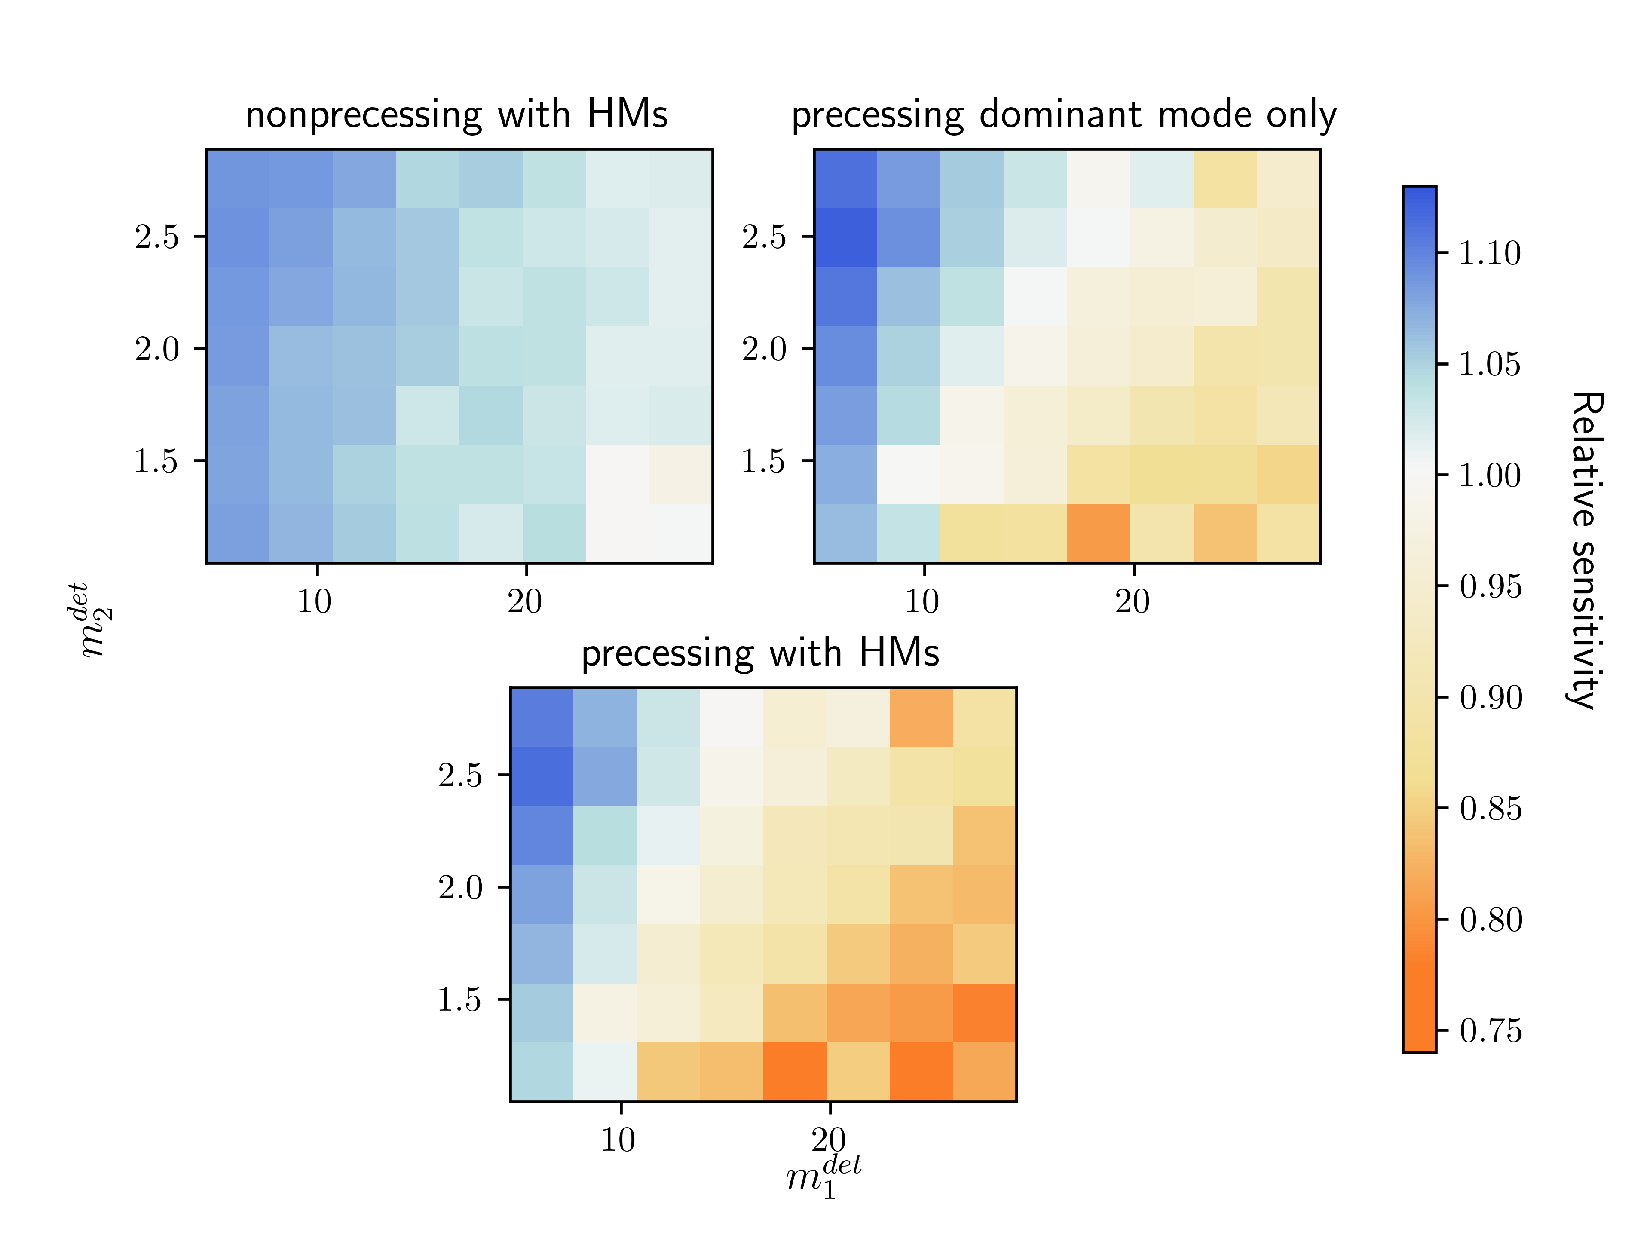
\includegraphics[width=13cm, height=10cm]{figures/HM_and_precession/aLIGO_weightedSRF.pdf}
        \caption{The fraction of precessing sources with HMs detected at a fixed false alarm rate relative to an idealized HM (upper left), dominant-mode precessing (upper right), or higher-mode precessing (lower) search as a function of the detector frame component masses $(m_1^{det}, m_2^{det})$. 
        We approximate the increase in background for the reference ideal searches by taking the relevant thresholds from \cite{Harry:2017weg, Harry:2016ijz} at a fixed FAR (as shown in table \ref{tab:FAR}). Regions with values $\geq 1$ indicate better sensitivity of a dominant mode, aligned-spin search relative to a search including additional effects, whereas, regions with modified SRF $< 1$ indicate lower relative sensitivity. We observe that a dominant mode, aligned spin search has better sensitivity than the naive idealized non-precessing search that includes HMs due to the increase in background; however the HM search will have higher sensitivity to edge-on sources. In the regions with $q > 6$, precessing searches will detect up to $\sim 20\%$ more signals for our fiducial signal
        population.}
        \label{fig:aLIGO_weightedSRF}
\end{figure*}

\begin{figure*}
        \centering
        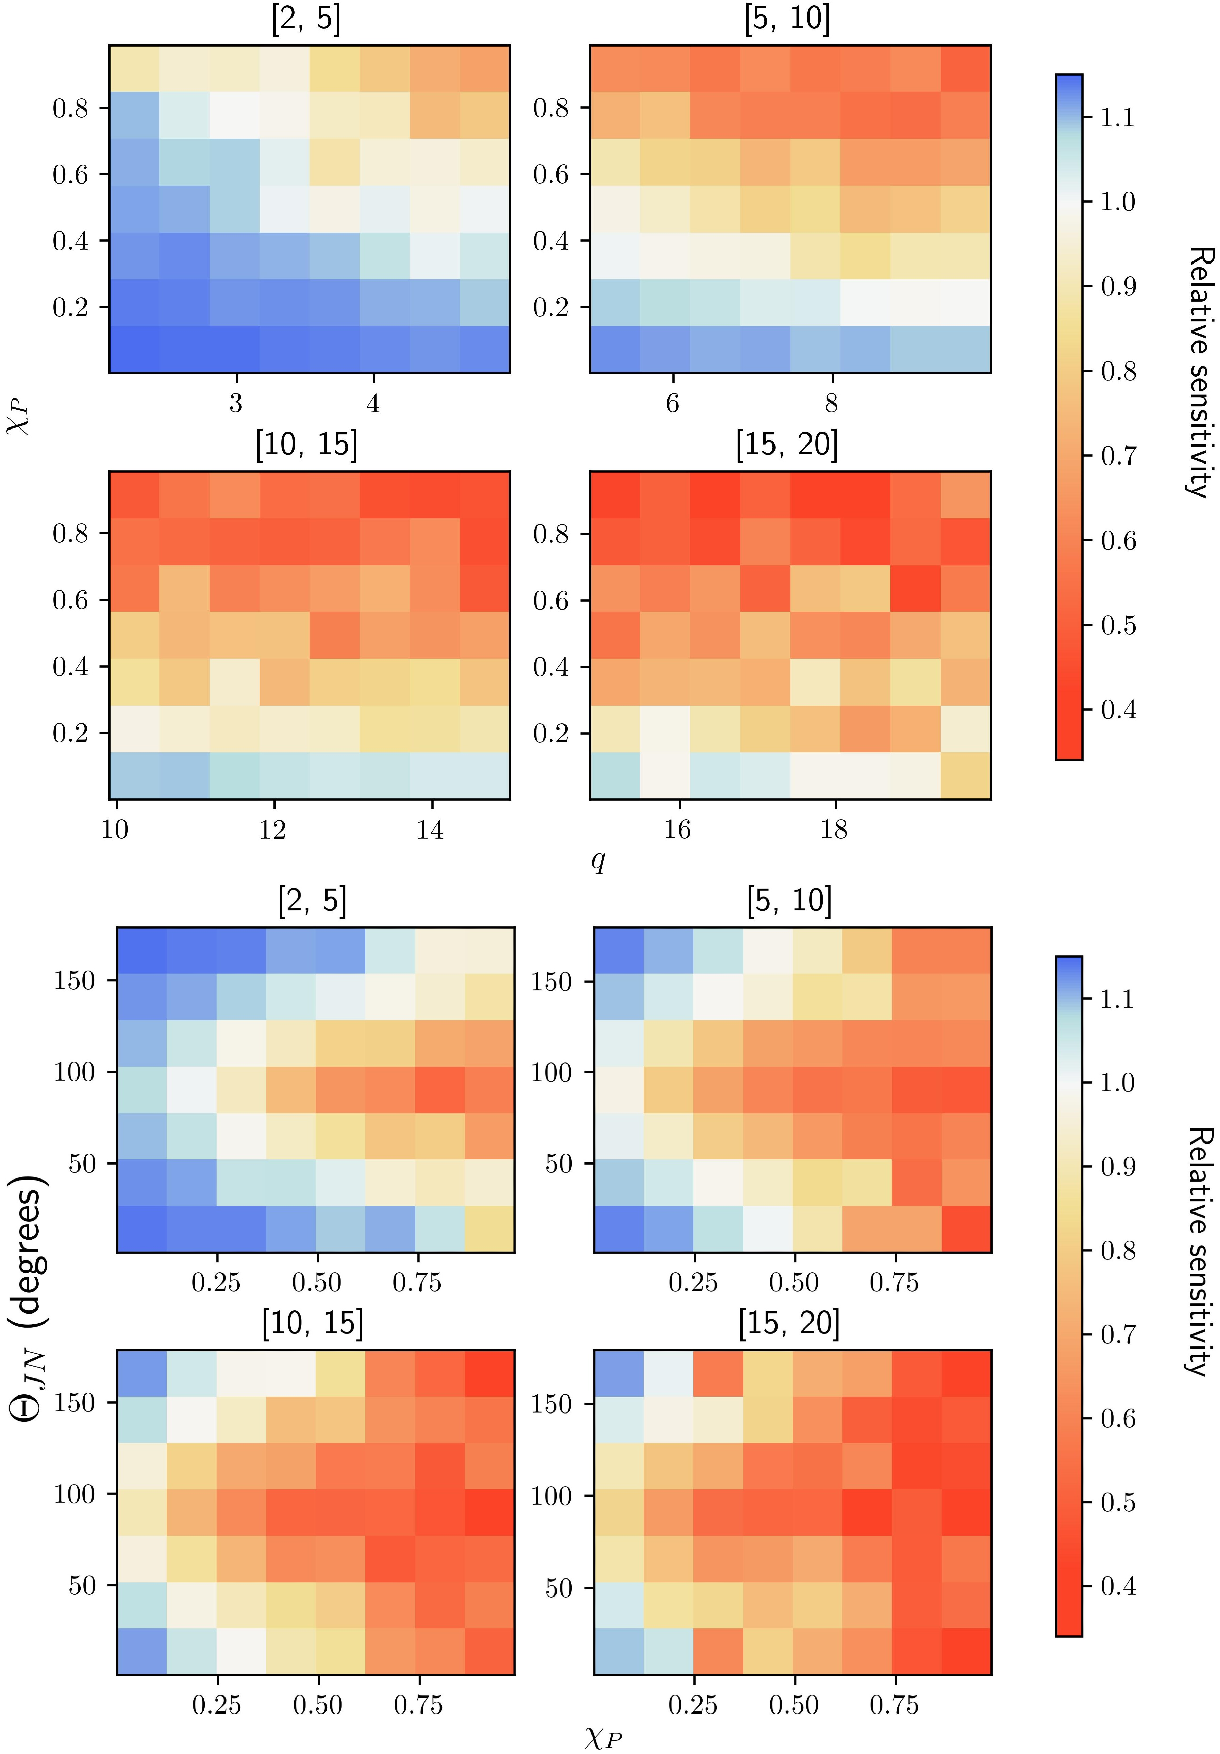
\includegraphics[width=0.85\linewidth]{figures/HM_and_precession/Merged.pdf}
        \caption{Relative sensitivity of an aligned-spin search w.r.t an idealized precessing search with HMs as a function of  $(q, \chi_P)$ (top) and $(\chi_{P}, \Theta_{JN})$ (bottom). Small mass-ratio $q \leq 5$ systems which are highly precessing will be missed by a dominant mode, aligned spin searches. For high mass-ratios $q > 6$, there will be a significant loss in sensitivity (up to $60\%$) even for moderately precessing systems.}
        \label{fig:merged}
\end{figure*}


\section{Developing a Fully Precessing Search}\label{sec:challenges}

Our results indicate a necessity to implement a precessing search for the identified regions of poor sensitivity. One way of implementing a precessing search could be to use the same statistic as Eq. (\ref{Eq:Simple-SNR-maximization}) and employ precessing templates. This approximation may not be valid while searching for signals with HMs or precession due to several reasons. For precessing signals, the two polarizations are not related by an overall phase shift $h_+ \not\propto i h_{\times}$, which is what enables the analytic maximization over extrinsic parameters. This is also true in the case of searching using HMs -- as each mode has a unique phase dependence $\Phi_{l,m}$. In the case of a precessing, higher-mode search, both the orbital phase and the inclination of binary, which are typically considered extrinsic parameters, would now behave as intrinsic parameters. The ideal search would marginalize over all extrinsic and intrinsic parameters coherently for all observing detectors. However, a naive implementation would be significantly more expensive than the aligned-spin search due to the increase in the number of intrinsic parameters (spin vectors, orbital phase, inclination), and the need to numerically marginalize over the extrinsic parameters. 

We can demonstrate the issue by comparing the match between the two polarizations $m(h_+, h_{\times})$ for every source in our population using precessing signals with HMs. The value (1 - $m(h_+, h_{\times})$) corresponds to the fraction of observed signal SNR lost as a result of approximation in Eq. (\ref{Eq:Simple-SNR-maximization}); a value of $m(h_+, h_{\times}) = 0.84$ corresponds to a loss of $16\%$. In Fig. \ref{fig:hplus_hcross}, we show the binned averaged value of the match as a function of ($\chi_P, \theta_{JN}$) at $f_{ref} = 100$ Hz. From the plot, we observe the standard analytical maximization of extrinsic parameters is valid for searching non-precessing systems except when they are nearly edge-on. However, when searching for precessing systems the match decreases with increasing $\chi_P$ or $\theta_{JN}$. We measure a loss in SNR up to $\sim 40-53\%$ for nearly edge-on and up to $\sim 10-40\%$ for face-on/off precessing binaries. These results clearly invalidate the approximation in Eq. (\ref{Eq:Simple-SNR-maximization}) and motivate the development of methods to efficiently marginalize over the extrinsic parameters of precessing sources.

Works have proposed new ways of approximating the optimal search statistic~\cite{Harry:2016ijz, Harry:2017weg}. These search methods maximise the SNR over fewer extrinsic parameters than in Eq. (\ref{Eq:Simple-SNR-maximization}) and across the remaining ones using a template bank with additional parameters; they also typically do this maximization incoherently between detectors. A generic approach to search for signals with HMs was introduced in \cite{Harry:2017weg}; the search maximised the SNR over ($d_L, \alpha, \delta, \psi$) and uses two additional parameters ($\iota, \Phi_c$) in the template bank. The same approach is employed in the first search for intermediate-mass BHs including HMs \cite{Chandra:2022ixv}. Similarly,~\cite{Harry:2016ijz} developed an approach to search for precessing signals; their statistic maximises the SNR over sky-parameters and imparts only one additional parameter to the template bank. 


\begin{figure}
    \centering
    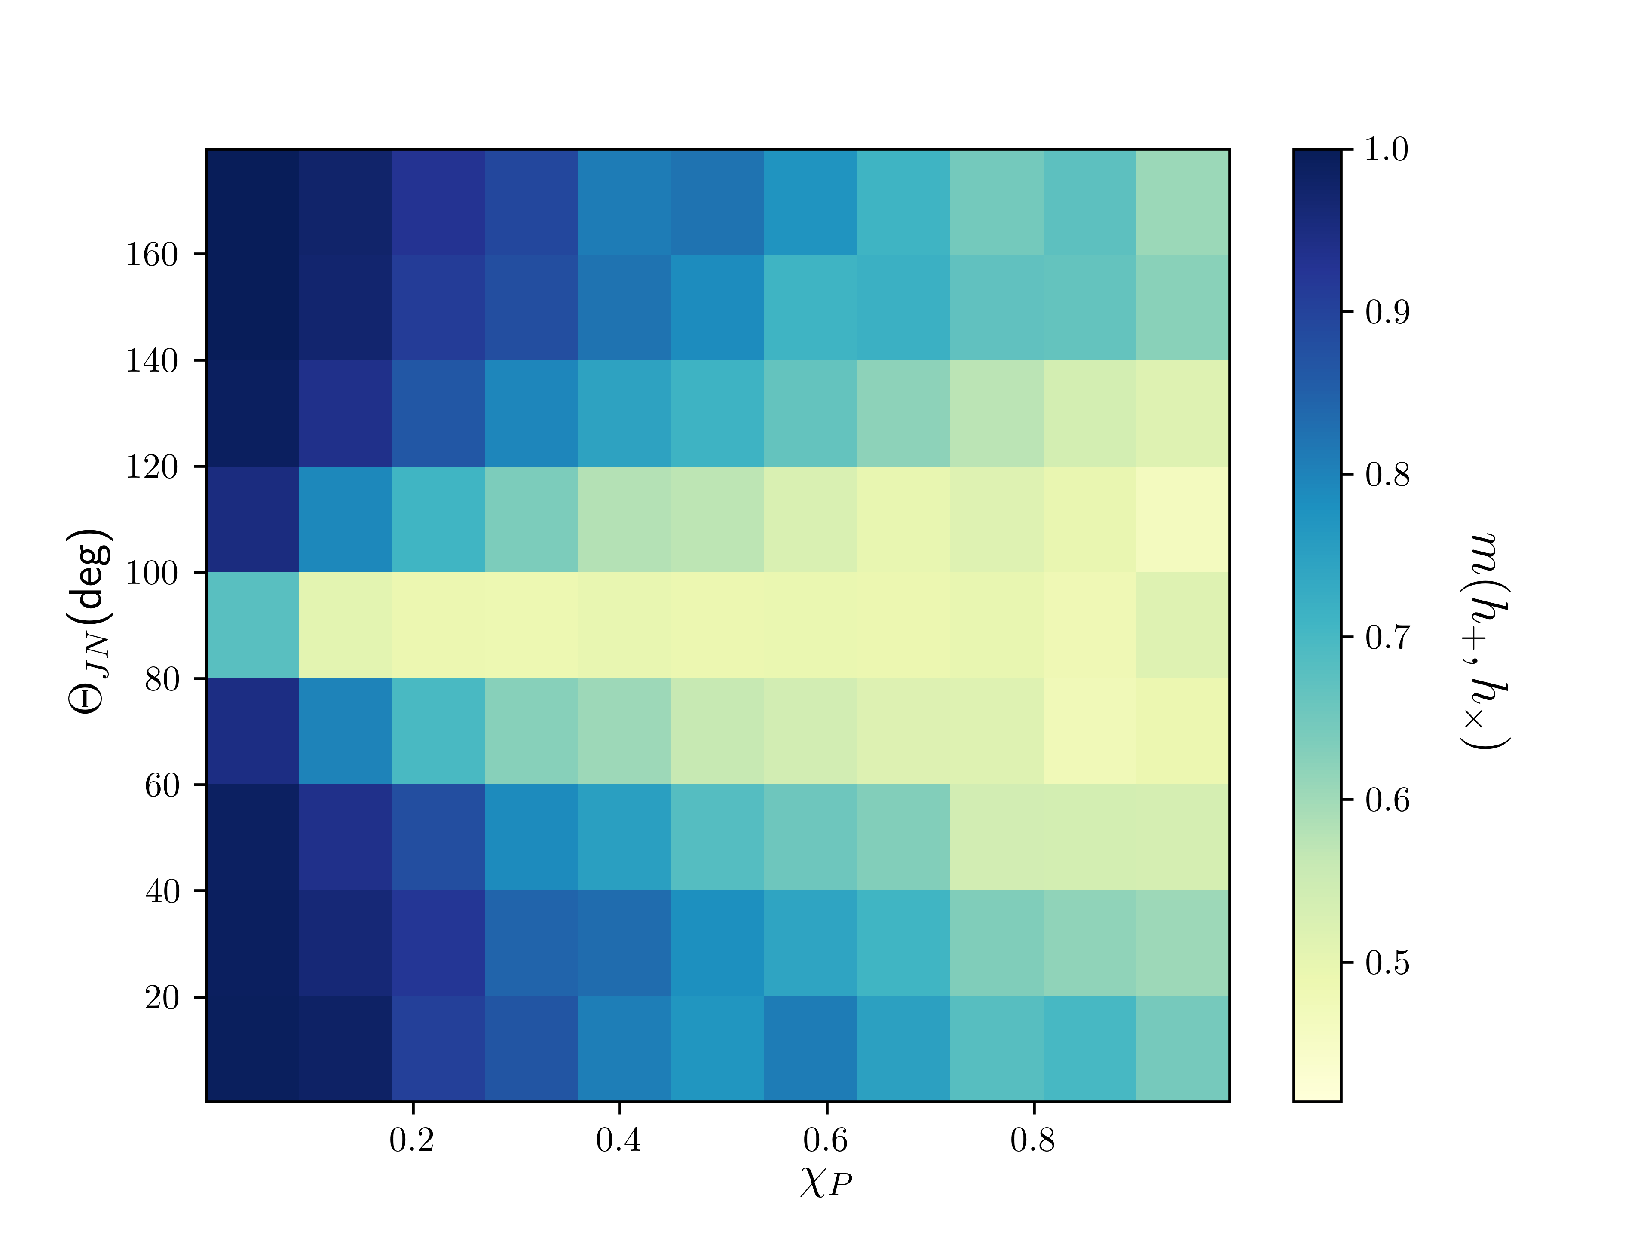
\includegraphics[width=\linewidth]{figures/HM_and_precession/hplus_hcross.pdf}
    \caption{ Distribution of match (overlap maximized over time and phase) between the two polarizations $m(h_{+},h_{\times})$ for a simulated population of precessing signals with higher modes across the two-dimensional surface $(\chi_P, \theta_{JN})$. The values correspond to the fractional loss in SNR measured using a single polarization matched filter statistic; regions with significantly lower values may require a generic statistic.} 
    \label{fig:hplus_hcross}
\end{figure}

\section{Conclusions and discussions}\label{sec:prec-conclusion}
In this work we have studied the sensitivity of dominant mode, aligned-spin searches, as have been employed in past gravitational-wave surveys ~\cite{LIGOScientific:2021djp, Olsen:2022pin, Nitz:2021uxj}, to a population of NSBH sources. We compare the number of sources an aligned spin search would detect at a fixed false alarm rate relative to idealized searches that incorporate either higher modes, precession, or both. In this study, we've used an estimate of the relative background of each search to account for the change in SNR threshold at a fixed false alarm rate; this could be further improved by a detailed study of precessing template bank generation, which we leave for future work.

We have modelled gravitational-wave signals using a recent waveform model which includes both the effects of precession and higher-order modes~\cite{Pratten:2020ceb}. The model has the largest potential systematics for highly precessing and asymmetrical-mass sources. While we do not expect qualitative changes to our results, improved models would help minimize potential systematic biases in precessing searches.

We find that the aligned spin searches are least effective in detecting sources with asymmetrical masses, large in-plane spins, or binaries with orientation close to edge-on. Dominant mode, aligned-spin searches lose up to $25\%$ of sources with mass-ratios $q > 6$ and up to $60\%$ of highly precessing systems $\chi_p > 0.5$. We compare four different noise curves -- Advanced LIGO design, A+, LIGO Voyager and Cosmic explorer and find that these results apply for each detector configuration we considered. 

Real detector data contains non-Gaussian transient noise~\cite{LIGOScientific:2016gtq, LIGO:2021ppb}; the impact of these artefacts is mitigated using a variety of vetoing methods~\cite{LIGOScientific:2017tza}, including signal consistency tests~\cite{Allen:2004gu, LIGOScientific:2017tza}. In this work we have not considered the impact of these vetoing methods. Since signal-consistency tests compare the expected signal to the data, it is possible that aligned-spin searches could misclassify signals with strong precession or HMs as noise. Therefore, we expect that in practice aligned-spin searches will have even stronger observational biases than presented here.

The detection of precessing systems or signals with higher-order modes provides better constraints of the component spins that carries signatures of the formation of compact-binary sources~\cite{Gompertz:2021xub, Stevenson:2017dlk, Talbot:2017yur, Rodriguez:2016vmx, Johnson-McDaniel:2021rvv}. We have identified regions of parameter space with significant bias against highly precessing systems. The poor sensitivity in these regions motivates the need to develop a search that can fully account for the gravitational-wave signal produced by precessing binaries. Precessing searches can pose computational challenges ~\cite{Harry:2016ijz} which might be overcome by implementing hierarchical strategies~\cite{Dhurkunde:2021csz, Soni:2021vls}. We expect that if we can solve these challenges, our results show that the solution will likely still apply for future detector configurations. Therefore, we strongly recommend a targeted precessing search in the identified regions with poor sensitivity.